\documentclass{article}
% if you need to pass options to natbib, use, e.g.:
%     \PassOptionsToPackage{numbers, compress}{natbib}
% before loading neurips_2024
% ready for submission
% \usepackage[nonatbib]{neurips_2024}

% to compile a preprint version, e.g., for submission to arXiv, add add the
% [preprint] option:
%     \usepackage[preprint]{neurips_2024}


% to compile a camera-ready version, add the [final] option, e.g.:
\usepackage[nonatbib, final]{neurips_2024}


% to avoid loading the natbib package, add option nonatbib:
%    \usepackage[nonatbib]{neurips_2024}



\usepackage[utf8]{inputenc} % allow utf-8 input
\usepackage[T1]{fontenc}    % use 8-bit T1 fonts
\usepackage{hyperref}       % hyperlinks
\usepackage{url}            % simple URL typesetting
\usepackage{circledsteps}
\usepackage{booktabs}       % professional-quality tables
\usepackage{amsfonts}       % blackboard math symbols
\usepackage{amsmath}
\usepackage{nicefrac}       % compact symbols for 1/2, etc.
\usepackage{microtype}      % microtypography
\usepackage{xcolor}         % colors
\usepackage{graphicx}
\usepackage{float}
\usepackage{multirow}
\usepackage{wrapfig}
\usepackage{enumitem}
\usepackage{listings}
% \usepackage[round,authoryear]{natbib}
% \bibliographystyle{plainnat}
% \usepackage{natbib}
% \usepackage{listings}
\makeatletter
\def\thanks#1{\protected@xdef\@thanks{\@thanks
        \protect\footnotetext{#1}}}
\makeatother
% unsrtnat
% \bibliographystyle{unsrtnat}
% \usepackage[authoryear]{natbib}






\title{Plan-on-Graph: Self-Correcting Adaptive Planning of Large Language Model on Knowledge Graphs}


% The \author macro works with any number of authors. There are two commands
% used to separate the names and addresses of multiple authors: \And and \AND.
%
% Using \And between authors leaves it to LaTeX to determine where to break the
% lines. Using \AND forces a line break at that point. So, if LaTeX puts 3 of 4
% authors names on the first line, and the last on the second line, try using
% \AND instead of \And before the third author name.

\author{Liyi Chen$^{1, 2 \dagger}$, Panrong Tong$^{2}$, Zhongming Jin$^{2}$, Ying Sun$^{3}$, Jieping Ye$^{2*}$, Hui Xiong$^{3, 4*}$ \\
$^{1}$ University of Science and Technology of China, 
$^{2}$ Alibaba Cloud Computing,\\
$^{3}$ Thrust of Artificial Intelligence, The Hong Kong University of Science and \\ Technology (Guangzhou), $^{4}$ Department of Computer Science and Engineering, \\The Hong Kong University of Science and Technology\\
\texttt{liyichencly@gmail.com, yings@hkust-gz.edu.cn, xionghui@ust.hk,}\\ \texttt{\{panrong.tpr, zhongming.jinzm, yejieping.ye\}@alibaba-inc.com}
\thanks{$\dagger$This work was accomplished when Liyi Chen was an intern at Alibaba Cloud Computing.}\thanks{*Corresponding authors.}}


\begin{document}


\maketitle


\begin{abstract}
Large Language Models (LLMs) have shown remarkable reasoning capabilities on complex tasks, but they still suffer from out-of-date knowledge, hallucinations, and opaque decision-making. 
In contrast, Knowledge Graphs (KGs) can provide explicit and editable knowledge for LLMs to alleviate these issues.
Existing paradigm of KG-augmented LLM manually predefines the breadth of exploration space and requires flawless navigation in KGs.
However, this paradigm cannot adaptively explore reasoning paths in KGs based on the question semantics and self-correct erroneous reasoning paths, resulting in a bottleneck in efficiency and effect.
To address these limitations, we propose a novel self-correcting adaptive planning paradigm for KG-augmented LLM named Plan-on-Graph (PoG), which first decomposes the question into several sub-objectives and then repeats the process of adaptively exploring reasoning paths, updating memory, and reflecting on the need to self-correct erroneous reasoning paths until arriving at the answer.
Specifically, three important mechanisms of \textit{Guidance}, \textit{Memory}, and \textit{Reflection} are designed to work together, to guarantee the adaptive breadth of self-correcting planning for graph reasoning. Finally, extensive experiments on three real-world datasets demonstrate the effectiveness and efficiency of PoG.
% To fully understand multiple conditions in complex questions and improve the accuracy of retrieval directions, we divide the questions into sub-questions that can be answered step by step. We also set up memory to record and update the answer status of sub-questions during the reasoning process, guiding the agent to plan the retrieval direction based on the information still needed to answer sub-questions.
% To address the non-adaptive breadth of retrieval, we dynamically prune and adjust the breadth of the retrieval using the semantic reasoning capabilities of large models. Additionally, by increasing the memory, we provide the possibility for self-correction. All the retrieved content is recorded in memory. If the breadth setting is too small, new retrieval paths can be supplemented based on the answer status of sub-questions in the memory.
% To increase fault tolerance, we have designed a mechanism of reflection at each layer of retrieval. This mechanism determines the retrieval direction based on the content in memory - whether to continue the retrieval along the planned path or to backtrack to the entities in previous steps
% and modify the retrieval path.

% we introduce a novel approach that combines the expansive knowledge and reasoning capabilities of Knowledge Graphs (KGs) with the advanced natural language understanding of LLMs, presenting a more flexible and fault-tolerant KG+LLM methodology. Unlike conventional methods that demand step-wise precision in reasoning, our approach leverages the robustness of KGs for factual information and utilizes LLMs for context-aware, nuanced understanding and question processing. 
% This synergy allows for the mitigation of errors emanating from the inherent imperfections of large models and the complex nature of natural language queries.

% Our KG+LLM framework dynamically interacts between the structured factual data within KGs and the adaptive, context-sensitive parsing and reasoning capabilities of LLMs. This results not only in enhanced accuracy in answering complex questions but also in significantly improved fault tolerance where the model can gracefully handle and recover from misunderstandings or errors in inference. 

% Preliminary evaluations of our approach against traditional LLM-based KBQA systems underscore its effectiveness, particularly in scenarios where nuanced comprehension and inferential reasoning are critical. This advancement heralds a more adaptable and resilient future for KBQA systems, promising to extend their applicability and reliability.
\end{abstract}

\vspace{-2mm}
\section{Introduction}
\vspace{-2mm}
\setcounter{footnote}{0}
% Notably, these models exemplified by ChatGPT~\cite{achiam2023gpt}, LLaMA~\cite{touvron2023llama}, and Mistral~\cite{jiang2023mistral} have become prominent pioneers in cutting-edge technological frontier, demonstrating a formidable aptitude for intricate semantic comprehension and reasoning.
Large Language Models (LLMs) have manifested outstanding performance in various natural language processing and data science tasks, such as question answering~\cite{wang2024t,li2024unigen,zhao2024comi}, text generation~\cite{ji2024chain, chen2023table, chen2023entity, gong2024graph}, recommender systems~\cite{zhang2023triple, zhang2024temporal, wu2024afdgcf, wang2024dynamic}, and domain-specific applications~\cite{tfwang-tsc-2023-hrl-acra, tfwang-ijcai-2024-flagvne, chen2024pre, wu2021linking, sun2024large}.
They leverage advanced deep learning techniques and immense amounts of pre-existing text data to understand and generate human language with impressive fluency and coherence.
Despite their success in numerous applications, LLMs still suffer from out-of-date knowledge, hallucinations, and opaque decision-making, highlighting the ongoing need for further investigation in this rapidly evolving field.

Intuitively, as large-scale structural knowledge bases, Knowledge Graphs (KGs)~\cite{bollacker2008freebase, auer2007dbpedia, chen2024tmea, wang2024unleashing} provide explicit and editable depictions of massive real-world knowledge, which have the potential to be a promising complement to the drawbacks of LLMs. 
 Previous studies manage to integrate KGs into LLM pre-training~\cite{zhang2019ernie, wang2021kepler} or fine-tuning~\cite{yao2019kg, luo2024reasoning} stage.
However, these methods mainly compress structured knowledge in KGs into LLMs' parameters in a black-box fashion and still cannot fully enhance the flexibility, reliability, and transparency of LLMs. 
Therefore, several attempts ~\cite{baek2023knowledge, axelsson2023using,wang2023boosting} first retrieve information from KGs and then deliver explicit knowledge into LLMs. Under these circumstances, LLMs do not directly participate in the graph reasoning process, making these methods excessively dependent on the KG completeness.
Recently, a KG-augmented LLM paradigm has been proposed to conduct graph reasoning, which treats the LLM as an agent to interactively explore related entities and relations on KGs and perform reasoning based on the retrieved knowledge.
% KGs and LLMs collaboratively work and complement each other's capabilities in each step of graph reasoning. 
% TODO 揉进去 这类范式定义检索的广度 并且 通过单向的检索得到子图。
For instance, StructGPT~\cite{jiang2023structgpt} and ToG~\cite{sun2024think} predefine the breadth of reasoning paths explored on the KG, and leverage the LLM to iterate the process of unidirectionally extending along the reasoning paths relevant to the question and reasoning the answer using these reasoning paths.
This KG-augmented LLM paradigm offers an opportunity for more comprehensively amalgamating the knowledge from both the KG and LLM by facilitating the step-by-step derivation of further insights.
% 新范式为什么好。 
% 要说为什么纠正很重要：有很多问题非常依赖这种自我纠正的机制。依赖的推理超出了这种范式能够搞定的。

% transfers input questions to machine-understandable command for KG searching and reasoning, but it does not participate in the graph reasoning process directly
% Many works designed knowledge-aware training objectives by incorporating KGs into the training data or leveraging KG prediction tasks as additional supervision.
% potentially be a promising complement to the drawbacks of LLMs.
% [TODO 这句写的不好]
% 早期工作
% 后来
% Therefore, some studies have attempted to incorporate KGs into LLM reasoning for question answering, which can be broadly categorized into semantic parsing and retrieval-augmented methods.
% Semantic parsing methods~\cite{li2023few, ye2022rng} harness LLMs to convert questions into logical queries and then execute them on KGs to obtain answers.
% , thereby generated logical queries are often non-executable and yield no answers due to mismatches with KGs.
% Retrieval-augmented methods~\cite{baek2023knowledge, axelsson2023using} search relevant subgraph information of KGs as the prompt to assist LLM in making judgements.
% making it difficult to provide correct responses when the KG lacks facts pertinent to the questions.
% However, these methods excessively rely on the LLMs' understanding of the question or factual evidence from KGs, lacks a deep integration of the LLM and KG during the reasoning process on the graph.
% For example, MindMap~\cite{wen2023mindmap} exploits LLMs to extract predefined-sized evidence subgraphs to build their own mind map that supports evidence-grounded generation, and reasons over the mind map to yield final outputs.
% RoG~\cite{luo2024reasoning} first generates relation paths grounded by KGs as faithful plans, and then uses these plans to retrieve top-K reasoning paths from the KGs for LLMs to conduct faithful reasoning.
% Because LLM does not know the structure and form of knowledge in the KG, it's difficult to effectively match the structure in the KG with the generated query statements.
% 早期的工作仅根据KG或者LLM中的信息推理答案，分为KG-only和LLM-only
% <有什么优势可以解决上述问题，因此一些工作开始了KG+LLM的结合>
% with vast factual knowledge provide a valuable external knowledge that can alleviate these issues of LLMs.
\begin{figure*}[t]
	\centering
	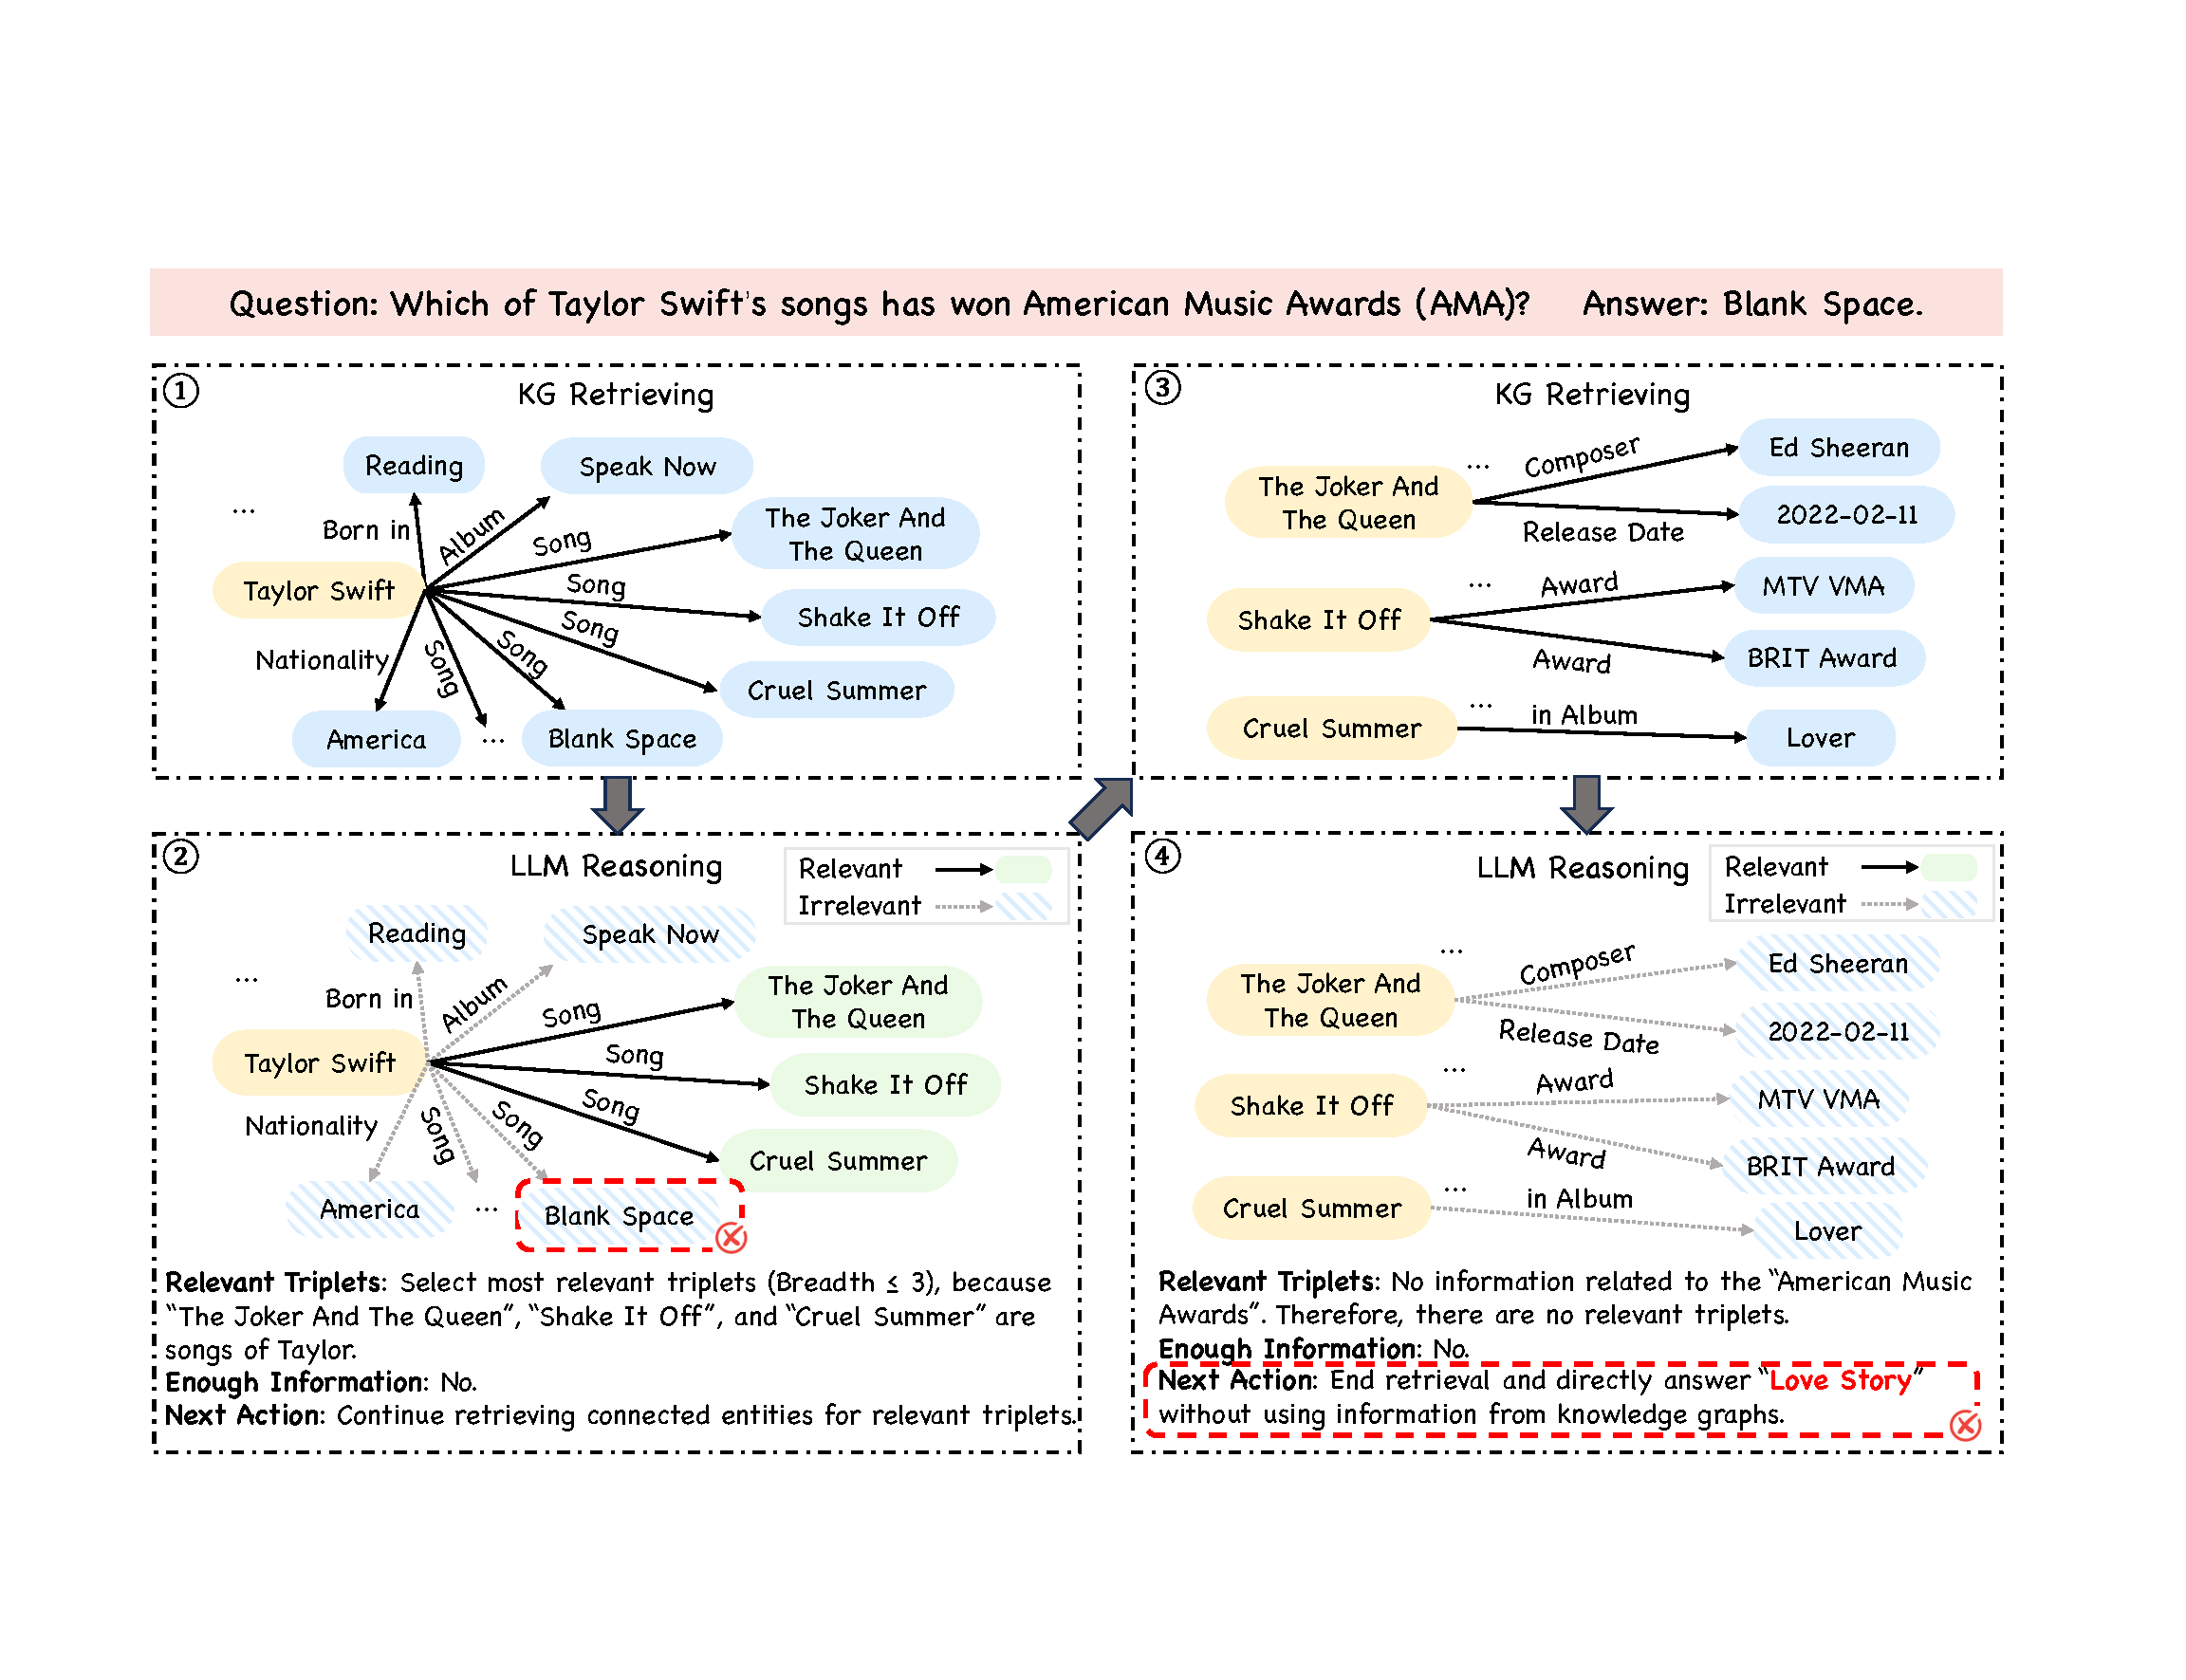
\includegraphics[width=\linewidth]{intro-cly.pdf}
        \setlength{\abovecaptionskip}{-2mm}
        \setlength{\belowcaptionskip}{-6mm}
	\caption{A toy example of existing KG-augmented LLM paradigm.}
	\label{Fig:intro}
\end{figure*}

% Although this KG-augmented LLM paradigm has achieved promising performance,
% TODO[一句话总结三个问题，图可能是会出现错误的，固定的广度无法召回] 存在一些问题可能导致会出现错误
% However, there are still many complex questions that cannot be resolved in the exploration all at once, leading to a heavy reliance on self-correction of erroneous reasoning paths.
% such as inferring relevance between the information available within the specified breadth and the question.
% When there is insufficient information to answer a question, LLM  will continue to extend current reasoning paths. 
However, existing paradigm may fail to plan the exploration of correct reasoning paths for many complex questions.
Figure~\ref{Fig:intro} illustrates an example of existing paradigm's limitations when answering the question ``Which of Taylor Swift's songs has won American Music Awards? (AMA)''. 
These limitations lie in:
(1) \textit{Predefined path breadth}: Existing paradigm requires manually setting the breadth of reasoning paths in KGs, and a fixed breadth may result in all the selected relations or entities being incorrect.
When determining the relevance between paths and questions in step \textcircled{2}, due to the limited maximum breadth of three and the uncertainty surrounding the respective awards of songs, the LLM selected maximum numbers of songs, ignoring the correct entity ``Blank Space''.
(2) \textit{Irreversible exploration direction}: 
The path exploration in existing paradigm is unidirectional without the ability to self-correct.
Even if the paths are incorrect, the LLM still continues to extend current incorrect paths and lead to the failure of reasoning on the KG.
In step \textcircled{3} and \textcircled{4}, since ``The Joker And The Queen'', ``Shake It Off'', and ``Cruel Summer'' were already chosen, the reasoning process continued on incorrect paths and the right answer was not found.
(3) \textit{Forgetting partial conditions}: 
During reasoning, the LLM may forget partial conditions in the question and cannot provide the answer that satisfies multiple conditions simultaneously.
In step \textcircled{4}, the LLM only remembered the condition that the song was by Taylor Swift but forgot the condition about the song winning an AMA award, leading to an incorrect answer, ``Love Story''.
Therefore, the reasoning of complex questions may heavily rely on adaptive exploration and self-correction of erroneous reasoning paths.
% lacks an effective mechanism for checking and correcting errors when the exploration is in the wrong reasoning paths. 
% [TODO] 对于复杂条件，只能关注一部分的条件，导致过程错误
% rendering it unreliable for verifying whether the reasoning path sufficiently answers the question. 
% TODO 这两个事很有必要，对于提升效率和效果
% In view of these limitations, we intend to explore reasoning paths in KGs with adaptive breadth based on the question semantics and self-correct the erroneous reasoning paths.


% In summary, this paradigm cannot adaptively explore reasoning paths in KGs based on the question semantics or self-correct when reasoning paths are wrong, resulting in a bottleneck in efficiency and effect improvement.
% 在思考时
% Failure to reason with multiple conditions in complex questions.
% it necessitates the manual predefinition of retrieval breadth and depends on LLMs' flawless navigation in KGs.
% As a result, they cannot adaptively explore the retrieval space based on the question semantics or self-correct when the reasoning path is wrong.

% 不同于以往的，弥补了xx问题，解决了xxx瓶颈。
% 现在的which后面是目标 不是方法。
% memory-guided self-correction
% why% memory-guided。KG上的一个reflection，图上做reflection的KG-Augmented LLM。为了做reflection，
To address these limitations, we propose a novel self-correcting adaptive planning paradigm for KG-augmented LLM named \textbf{P}lan-\textbf{o}n-\textbf{G}raph (\textbf{PoG}).
To the best of our knowledge, we are the first to design a reflection mechanism for self-correction and adaptive KG exploration into KG-augmented LLMs, effectively improving the ability and efficiency of LLM reasoning.
% which enhances reasoning path exploration with automatic breadth planning and self-correction of erroneous paths.
% LLM reasoning by finding factual evidence from the KG through adaptive breadth and self-correcting erroneous paths.
% exploits the LLM to plan KG exploration with flexible breadth and reflect to self-correct erroneous paths for enhancing the reasoning.
% automatically plan the path breadth based on question semantics and 
% To the best of our knowledge, we are the first to propose the reflection on the KG to achieve the self-correction in planning exploration.
% 提出了一个图上的self-correction，利用guidance
% [TODO] 我们是第一个提出在KG上做reflection
% explores the KG efficiently by adapting the breadth according to the semantics of the question and ensures effectiveness through self-correction mechanisms.
% [TODO] 三个机制和self-correction的关系
Specifically, PoG first decomposes the question into several sub-objectives as guidance for planning exploration, and then repeats the process of adaptively exploring reasoning paths to access relevant KG data, updating memory to provide dynamic evidence for reflection, and reflecting on the need to self-correct reasoning paths until arriving at the answer. In PoG,
three mechanisms are designed for adaptive self-correcting planning: (1) \textbf{Guidance}: To better guide adaptive exploration by harnessing conditions in the question, we employ the LLM to decompose the question into sub-objectives containing conditions, thereby benefiting the identification of relevant paths to each condition with flexible exploration breadth.
% Sub-objectives serve as the guidance of exploration, benefiting the LLM identifying relevant paths to each condition with flexible breadth.
% Sub-objectives serve as a guidance for exploration,
% mitigates the forgetting of partial conditions
% During the process, the sub-objectives and their completion status are recorded in memory, and then explicitly input into the LLM as the guidance for planning exploration and reflection.
% To thoroughly comprehend the multitude of conditions in complex questions and enhance the accuracy of reasoning retrieval direction, we first deconstruct the entire objective of the question into multiple sub-objectives that can be resolved step by step as guidance in the whole procedure. 
% 不会遗忘条件，既在检索和自我纠正 [self-correction] 更好的用问题中的关键条件来guide这个过程
% 为了显示的输入每个条件给大模型进行推理，存入memory，作为一个依据实现self-correction
% 根据子目标和子目标的实现情况作为planning的guidance
(2) \textbf{Memory}: The information stored in memory offers historical retrieval and reasoning information for reflection. 
% The retrieval subgraph, reasoning paths, and sub-objective status are dynamically recorded and updated in memory. 
% 子目标状态记录了和问题中的关键条件相关的已经推理出的信息，便于在reflection时规划仍需要探索的方向是continue还是correct。
% subgraph是为了将过去检索过的所有实体提供给LLM判断需要correct的位置
% Reasoning paths是为了保留图上实体间的关系给大模型推理答案并且基于修改.
We record and update the \textit{subgraph} to provide the LLM with all retrieved entities for initializing new exploration and self-correcting paths, \textit{reasoning paths} to preserve the relationships between entities for LLM reasoning and allow for path correction, and \textit{sub-objective status} to make the LLM recognize the known information of each condition and mitigate its forgetting in reflection stage.
% facilitating the planning of exploring information that still needs.
% records the information that has been inferred and is related to the key conditions in the question, facilitating the planning of whether to continue or correct the direction of exploration during reflection.
 % 根据子目标状态(子目标状态是guidance)来plan检索和反思，判断现有reasoning paths是否需要纠正，从subgraph中的实体开启新的探索。
% For supporting the flexible exploration and self-correction, 
% With memory, PoG can better plan exploration and reflection based on \textit{sub-objective status} to recognize already known information and what still need to explore, determine the need for self-correction of existing \textit{reasoning paths}, and initiate new exploration from the entities in the \textit{subgraph}.
% reflection分为评估和改正？
(3) \textbf{Reflection}: 
% To identify and rectify erroneous reasoning paths, we particularly design a reflection mechanism to determine whether and how to self-correct the KG exploration. 
To determine whether to continue or self-correct current reasoning paths, we design a reflection mechanism to employ the LLM to reason whether to consider other entities into new exploration and decide which entities to backtrack to for self-correction based on information in memory.
% After each step of path exploration, if the LLM judges that the current information is insufficient to answer the question, it will trigger reflection. 
% 根据memory中的信息，判断接下来要继续的exploration是否要考虑其他不在reasoning paths中的实体，和考虑哪一个实体
% 
% The reflection process involves the 
% LLM integrating the information summarized in memory to reason whether to consider other entities into new exploration and decide which entities to backtrack to for self-correction.
% in order to initiate new exploration
% The reflection process refers to the LLM integrating the information summarized in memory to assess whether there is a need to correct reasoning paths and decide the backtracked entity to initiate new exploration.
% determine the backtracking position of the previous entity, thus enabling the initiation of new exploration.
% The reflection refers that LLM integrates the  information summarized in memory to evaluate whether it needs to correct reasoning paths and decide previous entity's position to backtrack for initiating new exploration.
% [TODO] 一句话说明三个机制的总结
% 每个机制的内容要有和其他机制的关联
% 反思的是什么？看不出reflection依赖前面两个
% To enable self-correction of erroneous reasoning paths, relevant information from the KG is absorbed into the reasoning process of the LLM using memory. 
% After each step of path reasoning, the direction of exploration is assessed to determine whether to continue retrieving along the reasoning paths or to backtrack to previous steps and correct the reasoning paths.
% With information recorded in memory, 
Finally, extensive experiments on three real-world KGQA datasets validate the effectiveness and efficiency of PoG~\footnote{\url{https://github.com/liyichen-cly/PoG}}.
The main contributions of this paper are listed as follows:
\vspace{-0.2mm}
\begin{itemize}[leftmargin=1cm] 
    % which explores the KG efficiently by adapting the breadth according to the semantics of the question and ensure the effectiveness via the reflection for self-correction.  
    % based on conditions in the question
    \item We propose a novel self-correcting adaptive planning paradigm for KG-augmented LLM named PoG, which exploits the LLM to plan the adaptive breadth of reasoning paths and reflect to self-correct erroneous paths.
To the best of our knowledge, we are the first to incorporate a reflection mechanism for self-correction and adaptive KG exploration into KG-augmented LLMs, effectively augmenting the LLM's reasoning ability.
    % To the best of our knowledge, we are the first to propose the reflection on the KG as a means to achieve self-correction in planning exploration.
    % \vspace{-0.5mm}
    \item We specially design Guidance, Memory, and Reflection mechanisms for PoG. 
Guidance harnesses question conditions to better plan adaptive exploration by decomposing task into sub-objectives including conditions.
Memory records the subgraph, reasoning paths, and sub-objective status to provide historical retrieval and reasoning information for Reflection.
Based on Memory, Reflection reasons whether to self-correct reasoning paths and which entity to backtrack to for initiating new exploration.
    % PoG first harness conditions in the question to better guide the adaptive exploration process by decomposing the whole task into sub-objectives containing  conditions as Guidance through the LLM's semantic understanding.
    % Then, Memory and Reflection achieve self-correction collaboratively. Memory records the subgraph, reasoning paths, and sub-objective status to provide Reflection with a basis for assessing whether there is a need to correct reasoning paths and deciding which entity to backtrack to in order to initiate new exploration.
    % to collaboratively achieve the adaptive exploration breadth and self-correction.
    % \vspace{-0.5mm}
    % They work collaboratively
    \item We conduct extensive experiments on three real-world KGQA datasets, namely CWQ, WebQSP, and GrailQA. The results demonstrate not only the effectiveness but also the efficiency of our proposed novel PoG paradigm for KG-augmented LLM.
\end{itemize}
\vspace{-1.5mm}
% [TODO]claim contribution
% TODO: 为什么work，reflection的具体细节。说亮点
% 一句话说明，我们的设计能解决什么问题

% This allows the LLM to determine whether to continue retrieving along the reasoning path or to backtrack to previous steps and modify the reasoning path.

% two major mechanisms for graph reasoning are designed: memory and reflection.

 % seamlessly integrate KG and LLM in a collaborative reasoning, memory, and reflection manner. 
% Specifically, 
\vspace{-1mm}
\section{Preliminary}
\vspace{-2mm}
\textbf{Knowledge Graph (KG)} stores massive factual knowledge in the form of a set of triplets: $G = \{(e, r, e') \, | \, e, e' \in E, r \in R\}$, where $E$ and $R$ denote the set of entities and relations, respectively. 

\textbf{Relation Paths} are a sequence of relations: $z = \{r_1, r_2, ..., r_l\}$, where $r_i \in R$ denotes the $i$-th relation in the path and $l$ denotes the length of the path. 

% \textit{Example 1.} Given a relation path: $z = \text{marry\_to} \rightarrow \text{father\_of}$, a reasoning path instance could be: $w_z = \text{Alice marry\_to} \rightarrow \text{Bob father\_of} \rightarrow \text{Charlie}$, which denotes "Alice" is married to "Bob" and "Bob" is the father of "Charlie".

\textbf{Reasoning Paths} are the instances of a relation path $z$ in the KG: $p_z = e_0 \rightarrow r_1e_1 \rightarrow r_2e_2 \rightarrow... \rightarrow r_l e_l$, where $e_i \in E$ denotes the $i$-th entity and $r_i$ denotes the $i$-th relation in the relation path $z$.

\textbf{Knowledge Graph Question Answering (KGQA)} 
is the task of answering natural language questions based on a set of facts over the KG.
Given a question $q$, a knowledge graph $G$, and topic entities $T_q$ mentioned in $q$, the target of KGQA is to generate answers $A_q$ to the question $q$.
% is a typical reasoning task based on KGs. 
% Given a natural language question $q$ and a KG $G$, the target is to design a function $f$ to predict answers $a \in A_q$ based on knowledge from $G$, i.e., $a = f(q, G)$. 
Following previous studies~\cite{sun2024think}, 
we assume any entity $e_q \in T_q$ mentioned in $q$ and answers $a_q \in A_q$ are labeled and linked to the corresponding entities in $G$, i.e., $T_q, A_q \subseteq E$.

\vspace{-2.5mm}
\section{Methodology}
\vspace{-2mm}
\label{method}
\begin{figure*}[t]
	\centering
	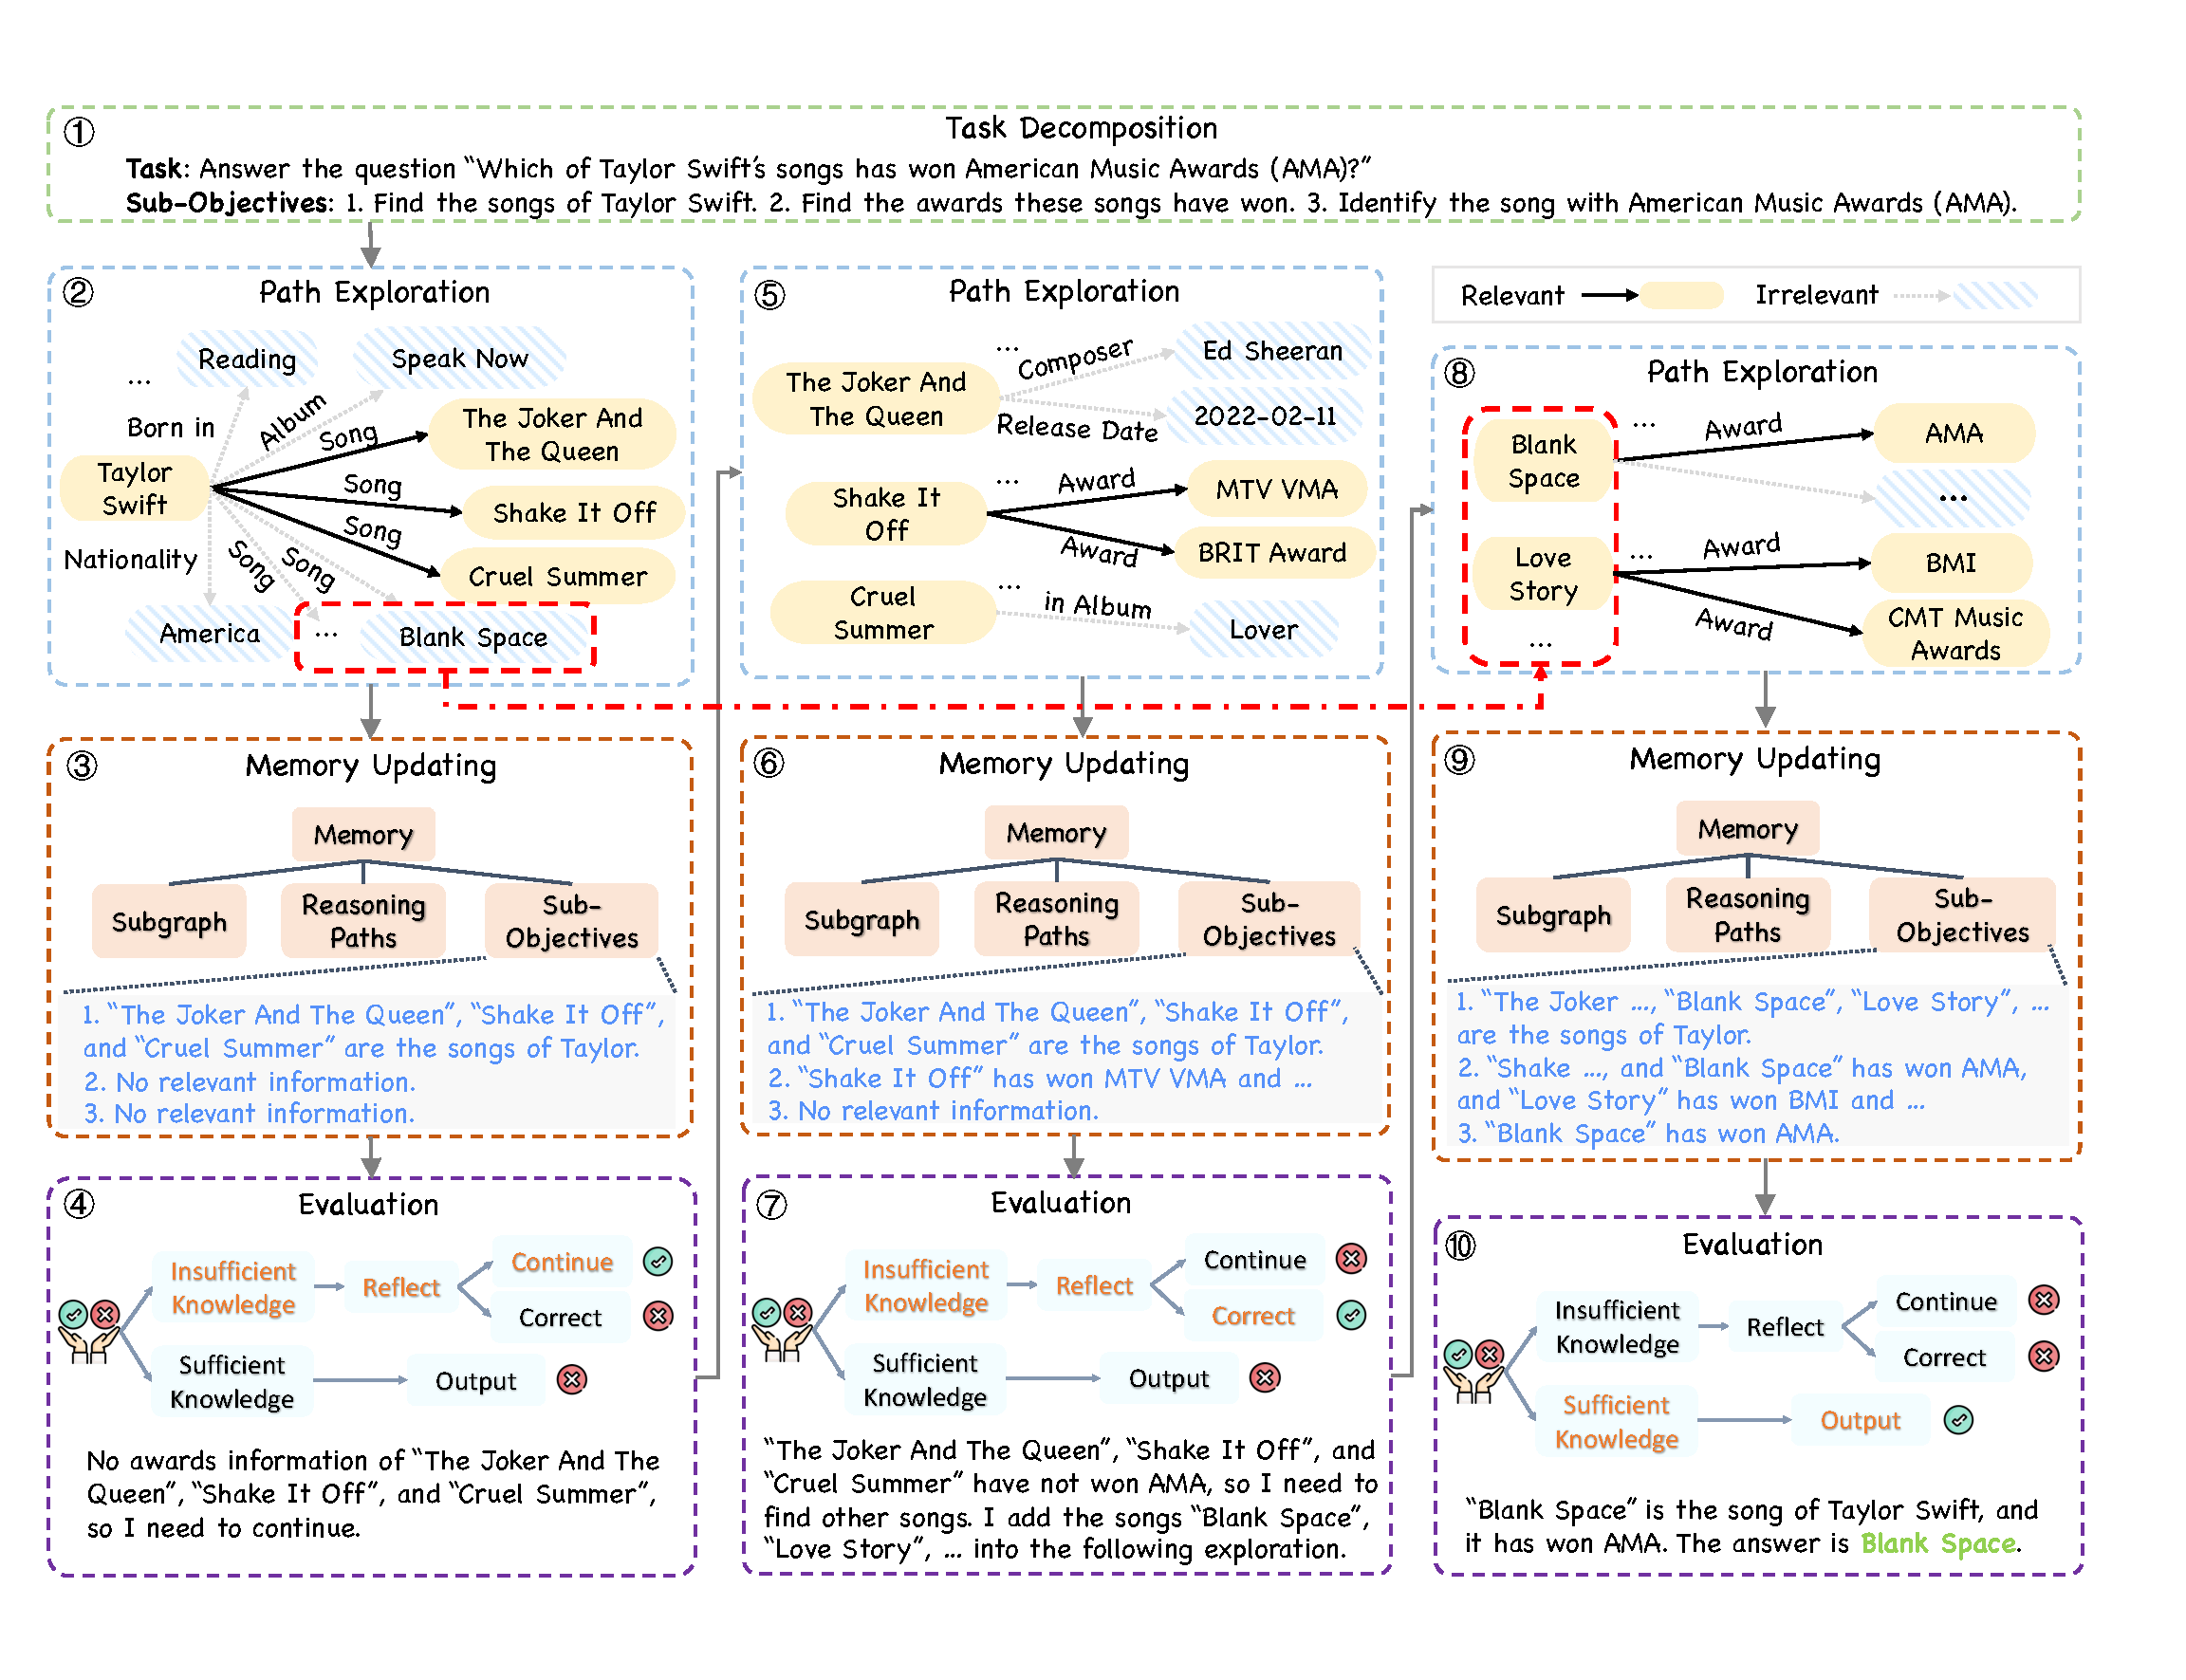
\includegraphics[width=\linewidth]{model-cly.pdf}
 % \vspace{-4mm}
        \setlength{\abovecaptionskip}{-2mm}
        \setlength{\belowcaptionskip}{-4mm}
	\caption{The framework overview of PoG, which includes four key components: Task Decomposition, Path Exploration, Memory Updating, and Evaluation.}
        % \vspace{-3mm}
	\label{Fig:framework}
\end{figure*}
% \subsection{Mechanism}
% \subsubsection{Guidance}
% \subsubsection{Memory}
% \subsubsection{Reflection}
% \subsection{Pipeline}
% [todo] what+why,每个之间的连接关系
In this section, we introduce the technical details of the novel self-correcting adaptive planning paradigm for KG-augmented LLM named Plan-on-Graph (PoG).
As illustrated in Figure~\ref{Fig:framework},
PoG consists of four key components: Task Decomposition, Path Exploration, Memory Updating, and Evaluation.
% \begin{itemize}
%     \item Task Decomposition
%     \item Path Exploration
%     \item Memory Updating
%     \item Evaluation
% \end{itemize}
% Specifically, PoG first decomposes the question into several sub-objectives and then repeats the process of exploring reasoning paths, updating memory, and evaluating the need of reflection for self-correction of reasoning paths until arriving at the answer.
PoG first decomposes the question into several sub-objectives as guidance of planning exploration and then repeats the process of adaptively exploring reasoning paths to access relevant KG data, updating memory to provide historical retrieval and reasoning information for reflection, and reflecting on the need to self-correct reasoning paths until arriving at the answer.
% The details of design are described in the following.
% 先进行task decomposition，然后再进行后面三个的迭代
\vspace{-2.5mm}
\subsection{Task Decomposition}
\vspace{-2mm}
To harness conditions in the question to better guide the adaptive exploration process, PoG decomposes the task of answering the question into multiple sub-objectives containing conditions through semantic analysis of the LLM. 
Sub-objectives serve as guidance for path exploration, benefiting the identification of relevant paths to each condition outlined in the question with flexible exploration breadth.
% At first, to thoroughly comprehend complex questions and enhance reasoning retrieval direction accuracy, 
% we decompose the task of answering the question into multiple achievable sub-objectives.
% These sub-objectives serve as a guide for the planning process and aid in addressing the all conditions outlined in the question.
Specifically, we prompt the LLM to decompose the original question $q$ into a list of sub-objectives for KG retrieval and reasoning. The prompt is shown in Appendix~\ref{prompt:td}.
The list of sub-objectives can be denoted as $O = \{o_1, o_2, o_3, ...\}$.
It is important to note that sub-objectives in $O$ may refer to the results obtained from other sub-objectives in $O$, allowing for interdependencies in the reasoning process.
% This decomposition allows for efficient handling of both graph-based retrieval and reasoning aspects, enhancing the overall performance of the model.
% These sub-objectives serve as guidance for planning and help address the multitude of conditions described in the question.
\vspace{-2mm}
\subsection{Path Exploration}
\vspace{-2mm}
% 为了开启图上的检索，首先需要找到图上路径的初始节点
We access relevant information from the KG by exploring reasoning paths in the KG.
On the initiation of path exploration, we localize the initial entities of reasoning paths, which correspond to the topic entities mentioned in the given question. Similar to prior research~\cite{jiang2023structgpt, sun2024think}, topic entities have been pre-identified and are part of the annotated datasets. 
Specifically, when presented with a question $q$, 
we use topic entities to serve as the initial elements of the reasoning paths, $E^0 = T_q = \{e^0_1, e^0_2, ..., e^0_{N_0} \}$, where $N_0$ is the number of topic entities.

% 在后续的迭代过程中，我们需要寻找到和问题相关的路径。以第D轮迭代为例，在迭代开始前，每条推理路径
In the subsequent iterations, we continue exploring reasoning paths most relevant to the question and suspend other reasoning paths.
Taking the $D$-th iteration as an example, before the iteration starts, each reasoning path $p_n \in P$ consists of $D_{p_n} (D_{p_n} \leq D - 1 )$ triplets, i.e., $p_n = \{(e^d_{s,n}, r^d_{j,n}, e^d_{o,n})\}_{d=1}^{D_{p_n}}$, where $e^d_{s,n}$ and $e^d_{o,n}$ denote subject and object entities, $r^d_{j,n}$ is a specific relation between them, $(e^d_{s,n}, r^d_{j,n}, e^d_{o,n})$ and $(e^{d+1}_{s,n}, r^{d+1}_{j,n}, e^{d+1}_{o,n})$ are linked to each other. 
% 我们只需要探索和问题最为语义相关的路径，暂停后续不相关的推理路径
It is noted that the length of each reasoning path may vary, because in the $D$-th iteration, we only continue exploring the reasoning paths most semantically relevant to the question, which are identified in the $D-1$-th iteration.
% TODO: 衔接的奇怪，想说用啥表示啥
The sets of tail entities and relations to be explored are denoted as $E^{D-1} = \{e^{D-1}_1, e^{D-1}_2, \dots, e^{D-1}_{N_{D-1}}\}$ and $R^{D-1} = \{r^{D-1}_1, r^{D-1}_2, \dots, r^{D-1}_{N_{D-1}}\}$, respectively, where $N_{D-1}$ is the length of $E^{D-1}$ and $R^{D-1}$.
% For distinguishing the reasoning paths,
We leverage the LLM to identify the most relevant entities $E^D$ from the neighboring entities of the current entity set $E^{D-1}$ based on the question $q$ and extend the reasoning paths $P$ with $E^D$.
% [TODO] 要说没有广度限制，而且有子目标的guidance
In order to manage the complexity of dealing with a large number of neighboring entities using the LLM, 
we propose an adaptive exploration strategy that is not limited by the fixed number of relations and entities. 
This strategy involves a two-step process of finding relevant relations and utilizing these selected relations to explore entities.
% we propose an two-step adaptive exploration strategy, involving finding relevant relations, and utilizing these selected relations to explore entities

\textbf{Relation Exploration.} Relation exploration is a process to retrieve the relations of all tail entities in $E^{D-1}$ and identify the most relevant relations to the question $q$ and the sub-objectives $O$.
To be specific, we first conduct the search to obtain all relations linked to the tail entities in $E^{D-1}$ as the candidate relation set $R^{D}_{cand} = \{r^{D}_{cand,1}, r^{D}_{cand,2}, ..., r^{D}_{cand, N_{D-1}}\}$. 
% where  $R^{D}_{cand,n}$ includes all relations connected to the tail entity $e_n^{D-1}$.
% The set of retrieval relations for all tail entities in $E_{D-1}$ is denoted as $R^{D}_{cand} = \{R^{D}_{cand,1}, R^{D}_{cand,2}, ..., R^{D}_{cand,N_{D-1}}\}$.
We utilize $R^{D}_{cand}$ to extend the reasoning paths into candidate reasoning paths $P_{cand}$. 
% 确定RD
Then, we employ the LLM to select a flexible number of 
% tails relations $R^{D}$, where $R^D_n\subseteq R^{D}_{cand,n}$
relevant reasoning paths $P$ ending with the tail relations in $R^{D}$ from $P_{cand}$, based on the semantic information of the question $q$, tail entities $E^{D-1}$, candidate relations $R^{D}_{cand}$, and sub-objectives $O$. 
The prompt is shown in Appendix~\ref{prompt:re}, and the pre-defined query for relation search is shown in Appendix~\ref{Apx:queryrel}.

% After retrieving the candidate relation sets $R^{D}_{cand}$ and obtaining the expanded candidate reasoning paths $P_{cand}$ from the relation retrieval, 

% The prompt used here can be found in Appendix E.3.1. 
% As shown in Figure 2, the LLM selects top-3 relations $\{\text{capital of}, \text{country}, \text{territory}\}$ out from all relations linked to the entity Canberra in the first iteration. Since Canberra is the only topic entity, the top-3 candidate reasoning paths are updated as $\{(\text{Canberra}, \text{capital of}),(\text{Canberra}, \text{country}),(\text{Canberra}, \text{territory})\}$


\textbf{Entity Exploration.} Analogously, entity exploration is a process to retrieve neighboring entities based on $R^{D}$ and $E^{D-1}$ and detect the most relevant entities to the question $q$. From the previous relation exploration, we obtain extended reasoning paths $P$ and new tail relations $R^D$. For each reasoning path $p_n \in P$, we can execute the queries of $(e_n^{D-1}, r_n^D, ?)$ or $(?, r_n^D, e_n^{D-1})$ to retrieve a candidate entity set $E^{D}_{cand,n}$, where $e_n^{D-1}$ and $r_n^D$ are the tail entity and relation in $p_n$.
When confronted with a large number of candidate entities, we use a small pre-trained DistilBERT~\cite{sanh2019distilbert}~\footnote{\url{https://huggingface.co/sentence-transformers/msmarco-distilbert-base-tas-b}}, to calculate the similarity between candidate entities and the question for recall.
Then, we summarize all candidate entity sets into $E^{D}_{cand}$ and use $E^{D}_{cand}$ as the tail entities to expand $P$ into $P_{cand}$.
With the candidate reasoning paths $P_{cand}$, we exploit the LLM to choose a flexible number of relevant reasoning paths $P$ ending with the tail entities $E^{D}$ from $P_{cand}$, based on the semantic information of the question $q$ and knowledge triplets composed of tail entities $E^{D-1}$, tail relations $R^D$ and candidate entities $E^{D}_{cand}$. The prompt is shown in Appendix~\ref{prompt:ee}, and the pre-defined query for entity search is shown in Appendix~\ref{Apx:queryent}.
% 延伸和丢弃

% Through conducting the relation and entity explorations presented above, we dynamically extend relevant paths and suspend irrelevant paths. The pre-defined queries are shown in Appendix~\ref{Apx:sparql}.
% increase the length of reasoning paths $P$ by 1,
% dynamically generate relevant reasoning paths $P$. 
% $p_n = e_0 \rightarrow r_1e_1 \rightarrow... \rightarrow r_{D-1} e_{D-1}$

% The retrieval procedure can be easily completed by executing two simple pre-defined formal queries shown in Appendix E.1 and E.2, which makes \textit{ToG} adapt well to different KGs without any training cost.

% In this step, PoG explores reasoning paths

% based on the sub-objectives decomposed previously. 

% It retrieves relevant information from the KG and combines it with the reasoning process of the LLM. By dynamically recording retrieval subgraphs, reasoning paths, and sub-objective completion status in the memory, the PoG model supports flexible retrieval and self-correction of reasoning.
\vspace{-2mm}
\subsection{Memory Updating}
\vspace{-2mm}
% The mechanism of Memory plays a crucial role in supporting the reflection for self-correcting erroneous reasoning paths. 
The information stored in memory provides historical retrieval and reasoning information for reflection. 
After a two-step exploration, we dynamically update the searched subgraph $G_{Sub}$, reasoning paths $P$, and sub-objective status $S$ in memory based on the ongoing reasoning process.

\textbf{Subgraph.} 
% 子图包含了所有检索过的关系和实体
The subgraph includes all retrieved relations and entities from the KG.
We update the subgraph in memory, which can be utilized during later reflection to determine which entity to backtrack to for self-correction.
% We update the subgraph in memory, which can be used to reason which entity to backtrack to in later reflection for self-correction.
% To provide all retrieved entities as candidates for initializing new exploration of reasoning path in self-correction,
% With the subgraph, LLM can determine which entity to backtrack to in later reflection stage.
In the $D$-th iteration, the searched subgraph $G_{Sub}$ is updated by adding the retrieved candidate relation set $R_{cand}^D$ and candidate entity set $E_{cand}^D$.

% after exploring new relations and entities, for the later
\textbf{Reasoning Paths.} 
In order to ensure that the LLM can understand relationships between entities for better reasoning and allow for path correction in reflection stage, we update reasoning paths $P$ to preserve the semantic structure within the KG.

\textbf{Sub-Objective Status.}
The LLM may forget partial conditions in the reasoning process. Sub-objectives obtained by decomposing the question can help the LLM remember multiple conditions in the question. 
The status of sub-objectives contains the current known information related to the sub-objectives,
which can aid the LLM in remembering the known information of each condition and determining whether to correct the exploration direction in reflection stage.
% rendering it unreliable for verifying whether reasoning paths sufficiently answer the question. 
Hence, we leverage the LLM to update the currently known information relevant to sub-objectives into sub-objective status $S = \{s_1, s_2, s_3, ...\},  |S| = |O|$, based on the semantic information of the question $q$, sub-objectives $O$, historical sub-objective status, and reasoning paths $P$, along with the LLM's own knowledge. 
The prompt is shown in Appendix~\ref{prompt:mu}.

\vspace{-2mm}
\subsection{Evaluation}
\vspace{-2mm}
% 经过了两步的探索和记忆的更新后，PoG就会利用大模型来评估当前已获取的信息（子问题状态、推理路径）是否足够得到答案。评估结果作为信号来触发反思。如果PoG认为信息充分，将结合推理路径、子问题状态、和自身的知识，推理出一个确切的答案。当信息不充分时，PoG根据推理路径、子问题状态、原计划下一迭代的实体来反思是否需要自我修改当前的推理路径：是沿着当前的推理路径继续探索，还是回溯到先前检索过的实体开启新的探索。

% After the path exploration and memory updating, PoG prompt the LLM to assess whether the current acquired information (sub-objective states, reasoning paths) is sufficient to infer an answer. 
% Due to the fact that the reasoning capability of LLM does not guarantee correctness of exploration all the time, there is a need for a mechanism to self-correct when errors occur. Therefore, we design a reflection mechanism to execute the self-correction.
% Specifially, the evaluation results serve as a signal to trigger the reflection. If the LLM believes the information is sufficient, LLM will integrate the reasoning path, sub-objective states, and its own knowledge to infer an exact answer. When the information is not sufficient, PoG will reflect on whether it needs to correct the current exploration direction based on sub-objective states and entities planned for the next iteration of retrieval in the memory:
% whether to continue exploring along the paths with tail entities $E^D$ or to backtrack to previously searched entities $E_{add}^D$ from $E_{cand} = E_{cand}^{1} \cup E_{cand}^2 \cup ... \cup E_{cand}^D$ and add the new exploration for the correction.
% If it is determined that a correction is necessary, we will add \(E_{\text{add}}^D\) to \(E^D\), i.e., $E^D= E^D \cup E_{add}^D$.

After the path exploration and memory updating, PoG prompts the LLM to reason whether the current acquired information, including sub-objective states and reasoning paths recorded in memory, is sufficient to infer an answer. 
The prompt is shown in Appendix~\ref{prompt:aq}.
If the LLM determines that the information is sufficient, it will integrate reasoning paths, sub-objective states, and its own knowledge to provide an answer.
When information is considered insufficient, there may be two situations. One is that PoG will acquire sufficient information after further extension of current paths, and the other is that current paths are incorrect.
% While the information is deemed insufficient,
Since the reasoning capability of the LLM does not always guarantee the correctness of path exploration, there is a need to self-correct erroneous reasoning paths. 
Therefore, we design a reflection mechanism to determine whether and how to self-correct reasoning paths.
% 当llm认为信息不充分时，让llm进入反思的阶段
When the LLM believes that the information is insufficient, PoG enters the stage of reflection.
Specifically, PoG utilizes the LLM to reflect on whether to correct the current exploration direction based on the question $q$, sub-objective status $S$, reasoning paths $P$, and entities planned for the next iteration of retrieval $E^D$ from memory. Besides, the LLM will provide the reason for the reflection result.
% 如果大模型认为除了E^D中的实体，还有必要添加其他的实体来进行探索，那就需要correct。否则，就沿着当前的推理路径继续延伸。
If the LLM judges that it is necessary to incorporate additional entities beyond those in $E^D$ for exploration, then a self-correction of reasoning paths is needed. Otherwise, PoG will continue exploring along the current reasoning paths with tail entities in $E^D$.
For self-correction, PoG employs the LLM to decide which entities in \(E_{\text{cand}} = E_{\text{cand}}^{1} \cup E_{\text{cand}}^2 \cup ... \cup E_{\text{cand}}^D\) to backtrack to based on sub-objective states in $S$ and the reason for additional retrieval obtained from the reflection, and adds new exploration of backtracked entities \(E_{\text{add}}^D\) into \(E^D\) for the self-correction, denoted as \(E^D= E^D \cup E_{\text{add}}^D\).
 The prompts for reflection are shown in Appendix~\ref{prompt:reflection}.
 % If it is determined that a correction is necessary, we will add \(E_{\text{add}}^D\) into \(E^D\), denoted as \(E^D= E^D \cup E_{\text{add}}^D\).
% 不足够得到所有有用信息，
% Specifically, the evaluation results serve as a signal to trigger the reflection. 
% If the LLM determines that the information is sufficient, it will integrate the reasoning paths, sub-objective states, and its own knowledge to infer an exact answer. 
% While the information is deemed insufficient, PoG will reflect on whether it needs to correct the current exploration direction based on sub-objective states in $S$ and entities planned for the next iteration of retrieval $E^D$ from the memory. 
% This involves deciding whether to continue exploring along the paths with tail entities \(E^D\), or to backtrack to previously searched entities from \(E_{\text{cand}} = E_{\text{cand}}^{1} \cup E_{\text{cand}}^2 \cup ... \cup E_{\text{cand}}^D\), and add new exploration of backtracked entities \(E_{\text{add}}^D\) for the correction.
% If it is determined that a correction is necessary, we will add \(E_{\text{add}}^D\) into \(E^D\), denoted as \(E^D= E^D \cup E_{\text{add}}^D\).

% [opt] 效率优化，下一阶段的topic ent做筛选
% , PoG assesses 
% the direction of retrieval to determine whether to continue along the reasoning paths or to backtrack and modify them based on the current progress. This reflection mechanism enables self-correction of erroneous reasoning paths by incorporating relevant information from the KG into the reasoning process of the LLM.
% This allows for efficient modification and adaptation of reasoning paths as new information is encountered. 

\vspace{-2mm}
\section{Experiments}
\label{experiment}
\vspace{-2mm}
% In this section, we present extensive experiments conducted on three real-world datasets. 
% We first describe the setups of our experiments, and then provide the experimental results to demonstrate not only the effectiveness and but also the efficiency of PoG.
% More details and results of experiments are provided in Appendix~\ref{apdx:exp}. 
% \vspace{-1mm}
\subsection{Experimental Setups}
\label{setup}
\vspace{-1mm}
\subsubsection{Datasets \& Evaluation Metrics}
\vspace{-2mm}
To demonstrate the effectiveness of PoG on complex reasoning over knowledge graphs, we adopt three representative multi-hop KGQA datasets: CWQ~\cite{talmor2018web}, WebQSP~\cite{yih2016value}, and GrailQA~\cite{gu2021beyond}.
All three datasets rely on the external knowledge graph from Freebase~\cite{bollacker2008freebase}.
For the large dataset GrailQA, we utilize the same testing samples as those in ToG~\cite{sun2024think} to improve computational efficiency.
Following prior research~\cite{li2023few, jiang2023structgpt, sun2024think}, we use exact match accuracy (Hits@1) as the evaluation metric.

% Since our proposed PoG does not require training, we only use the test sets of these datasets.
% \subsubsection{}
\vspace{-2mm}
\subsubsection{Comparison Methods}
\vspace{-2mm}
% TODO 话很奇怪
Due to variations in the performance of the method across different datasets, we select prior state-of-the-art (SOTA) approaches as baselines for each dataset.
They can be categorized into two groups: (1) \textit{LLM-only methods}, including standard prompting (IO prompt)~\cite{brown2020language}, Chain-of-Thought prompting \begin{wraptable}[25]{r}{7cm}
\small
\centering
\vspace{-4mm}
\caption{Performance comparison of different methods on CWQ and WebQSP.}
\label{Tab:maincw}
\setlength{\tabcolsep}{0.5mm}{\begin{tabular}{lcc}
\toprule
\textbf{Method}  & \textbf{CWQ} & \textbf{WebQSP}  \\ \midrule
\multicolumn{3}{c}{\textit{LLM-Only}} \\ \midrule
IO Prompt~\cite{brown2020language}&37.6&63.3\\
CoT~\cite{wei2022chain}&38.8&62.2\\
SC~\cite{wang2023self}&45.4&61.1\\
\midrule
\multicolumn{3}{c}{\textit{Fine-Tuned KG-Augmented LLM}} \\ \midrule
UniKGQA~\cite{jiang2023unikgqa} & 51.2 & 79.1\\
% CBR-KBQA~\cite{} & 67.1 & -\\
TIARA~\cite{shu2022tiara} & -&75.2\\
RE-KBQA~\cite{cao2023pay} & 50.3 & 74.6\\
% FC-KBQA~\cite{zhang2023fc} & 56.4 & 76.9\\
DeCAF~\cite{yu2023decaf} & 70.4&82.1\\
RoG~\cite{luo2024reasoning} & 62.6&85.7\\
% ChatKBQA~\cite{} & 77.8&79.8\\
 \midrule
\multicolumn{3}{c}{\textit{Prompting KG-Augmented LLM w/GPT-3.5 or others}} \\ \midrule

KD-CoT~\cite{wang2023knowledge}& 50.5 &73.7 \\
KB-BINDER~\cite{li2023few}&-&74.4\\
StructGPT~\cite{jiang2023structgpt} & 54.3 & 72.6\\
ToG~\cite{sun2024think}& 57.1&76.2\\
\textbf{PoG}& \textbf{63.2} &  \textbf{82.0}   \\
\midrule
\multicolumn{3}{c}{\textit{Prompting KG-Augmented LLM w/GPT-4}}\\
\midrule
InteractiveKBQA~\cite{xiong2024interactive} & 59.2 &72.5\\
ToG~\cite{sun2024think} & 67.6 &82.6 \\
\textbf{PoG}   & \textbf{75.0} &\textbf{87.3}                     \\ \bottomrule
\end{tabular}}
% \end{table}
\end{wraptable}(CoT)~\cite{wei2022chain},
and Self-Consistency (SC)~\cite{wang2023self}. 
(2) \textit{KG-augmented LLM methods}, including fine-tuned and prompting methods. 
For CWQ and WebQSP, we utilize UniKGQA~\cite{jiang2023unikgqa}, TIARA~\cite{shu2022tiara}, RE-KBQA~\cite{cao2023pay}, DeCAF~\cite{yu2023decaf}, and RoG~\cite{luo2024reasoning} as fine-tuned baselines and KD-CoT~\cite{wang2023knowledge}, KB-BINDER~\cite{li2023few}, StructGPT~\cite{jiang2023structgpt}, Interactive KBQA~\cite{xiong2024interactive}, and ToG~\cite{sun2024think} as prompting baselines. For GrailQA, we utilize RnG-KBQA~\cite{ye2022rng}, TIARA~\cite{shu2022tiara}, FC-KBQA~\cite{zhang2023fc}, Pangu~\cite{gu2023don}, FlexKBQA~\cite{li2024flexkbqa}, and GAIN~\cite{shu2024distribution} as fine-tuned baselines and KB-BINDER~\cite{li2023few} and ToG~\cite{sun2024think} as prompting baselines.
The descriptions of baselines are presented in Appendix~\ref{Apd:baseline}.
% For each dataset, we select prior state-of-the-art (SOTA) approaches on it. 
% TODO: 要全部列举吗

% \vspace{-2mm}
\subsection{Performance Comparison}
\vspace{-2mm}
We compare PoG with the SOTA baselines to demonstrate its effectiveness for KG-augmented LLM.
Table~\ref{Tab:maincw} and Table~\ref{Tab:maing} present the experimental results on CWQ, WebQSP, and GrailQA datasets. 
Overall, PoG achieves the best performance across all three datasets.
Specifically, we can make the following observations.
First, compared to all prompting KG-augmented LLM baselines, PoG shows superior performance advantages. Regardless of whether GPT-3.5 or GPT-4 is used as the underlying LLM, PoG substantially outperforms the SOTA baseline, ToG.
ToG explores reasoning paths with a fixed exploration breadth and cannot detect or correct the errors, showing limitations in effect and efficiency. Meantime, we specially design self-correction and adaptive planning mechanisms, which can effectively improve both performance and efficiency.
Second, although PoG is a training-free prompting method, its performance is highly competitive with fine-tuned KG-augmented LLM baselines. When using GPT-4, the performance of PoG exceeds all fine-tuned KG-augmented LLM baselines across the board. Even with GPT-3.5,  the result of PoG on GrailQA surpasses all fine-tuned KG-augmented LLM methods.
% Fine-tuned methods require training and utilize considerable computational resources and time for planning and reasoning optimization. 
This suggests that our designed guidance, memory, and reflection mechanisms allow PoG's effect to surpass most of the fine-tuned methods.
Third, the improvement of PoG is obvious when compared to LLM-only baselines, which do not leverage external KGs. Besides, all KG-augmented LLM methods consistently outperform LLM-only methods, indicating the value of incorporating KGs to enhance LLM performance. Moreover, PoG further improves the effectiveness of KG-augmented LLMs through its self-correctable adaptive planning.
Additionally, it is worth noting that PoG with GPT-3.5 outperforms other methods on the zero-shot subset of the GrailQA dataset by a large margin, apparently outperforming all fine-tuned KG-augmented LLMs on this category. The self-correction mechanism in PoG allows it to dynamically correct errors during the reasoning process, which is crucial for zero-shot problems.



% Please add the following required packages to your document preamble:
% \usepackage{booktabs}
% \usepackage{multirow}
\begin{table}[t]
\small
% \setlength{\abovecaptionskip}{-2mm}
\setlength{\belowcaptionskip}{-0.1mm}
\caption{Performance comparison of different methods on GrailQA.}
\label{Tab:maing}
\centering
\begin{tabular}{lcccc}
\toprule
\multicolumn{1}{c}{\multirow{2}{*}{\textbf{Method}}}               & \multicolumn{4}{c}{\textbf{GrailQA}}                              \\ \cmidrule(l){2-5} 
\multicolumn{1}{c}{}                                               & \multicolumn{1}{l}{\textbf{Overall}} & \textbf{I.I.D.} & \textbf{Compositional} & \textbf{Zero-shot} \\ \midrule
\multicolumn{5}{c}{\textit{LLM-Only}} \\ 
\midrule
IO Prompt~\cite{brown2020language}&29.4&-&-&-\\
CoT~\cite{wei2022chain}&28.1&-&-&-\\
SC~\cite{wang2023self}&29.6&-&-&-\\  
\midrule
\multicolumn{5}{c}{\textit{Fine-Tuned KG-Augmented LLM}}                                                                                               \\ \midrule
RnG-KBQA~\cite{ye2022rng} & 68.8&86.2&63.8&63.0\\
TIARA~\cite{shu2022tiara} & 73.0&87.8&69.2&68.0\\
% ArcaneQA~\cite{gu2022arcaneqa} & 63.8&85.6&65.8&52.9\\
FC-KBQA~\cite{zhang2023fc}&73.2&88.5&70.0&67.6\\
% DeCAF~\cite{yu2023decaf}                    & 68.4  &  84.8   &   73.4     &     58.6      \\
Pangu~\cite{gu2023don} & 75.4&84.4&74.6&71.6\\
FlexKBQA~\cite{li2024flexkbqa} &62.8&71.3&59.1&60.6\\
GAIN~\cite{shu2024distribution} & 76.3&88.5&73.7&71.8\\
 \midrule
\multicolumn{5}{c}{\textit{Prompting KG-Augmented LLM w/GPT-3.5 or others}}             \\            
\midrule
KB-BINDER~\cite{li2023few}&50.6&-&-&-\\
% StructGPT~\cite{jiang2023structgpt}    & 52.6&  -&   -  & -\\
ToG~\cite{sun2024think}&                            68.7 &  70.1   &   56.1 &   72.7    \\
\textbf{PoG}&\textbf{76.5}&\textbf{76.3}&\textbf{62.1}&\textbf{81.7} \\ \midrule
\multicolumn{5}{c}{\textit{Prompting KG-Augmented LLM w/GPT-4}}                                                                                        \\ \midrule
ToG~\cite{sun2024think}&81.4 & 79.4&67.3&86.5 \\
\textbf{PoG}&\textbf{84.7}&\textbf{87.9}&\textbf{69.7}&\textbf{88.6}\\ \bottomrule
\end{tabular}
\vspace{-2mm}
\end{table}

% In summary, the experimental results clearly demonstrate the superiority of our proposed PoG method, which not only outperforms strong prompting KG-augmented LLM baselines but also competes favorably with and, in many cases, exceeds the performance of fine-tuned models, highlighting its effectiveness and efficiency in leveraging external knowledge graphs to enhance LLM capabilities.

% Table~\ref{Tab:maincw} and Table~\ref{Tab:maing} present the experimental results of the performance comparison of different models on CWQ, WebQSP, and GrailQA datasets. From the overview, our proposed PoG achieves the best performance on all three datasets.
% Specifically, we have the following findings. First, compared with all prompting KG-augmented LLM baselines, PoG demonstrates significant advantages. Regardless of which LLM is used (GPT-3.5 or GPT-4), PoG far surpasses the performance of the strongest baseline, ToG.
% Second, even though PoG is a training-free prompting method, its performance can compete with fine-tuned baselines. With GPT-4, the performance outperforms all fine-tuned baselines, and with GPT-3.5, the result on GrailQA also exceeds all fine-tuning methods.
% Third, the advantages of PoG are more pronounced in comparison to LLM-only baselines, and all KG-augmented methods perform better than LLM-only methods. This indicates that leveraging KG to enhance LLM is a valuable approach, and our designed PoG further improves the effectiveness for KG-augmented LLM by self- correctable adaptive planning.
% 1.和所有的prompting方法相比，PoG表现出了显著的优势。无论是在哪个LLM(gpt3.5/gpt4)，都远超最强的baseline ToG的效果。2.即使PoG是一个无须训练的prompting方法，它的效果也能够和微调方法比上一比。with GPT4的效果能够超过了所有的微调方法，并且withGPT3.5在GrailQA上的结果就能够超过了所有的微调方法。 3.和LLM-Only方法相比，PoG的优势更加明显，并且所有的KG-Augmented方法都超过了LLM-Only。说明用KG来增强LLM是一个有价值的方式，我们设计的PoG又进一步的提升了效果。


\vspace{-2mm}
\subsection{Ablation Study}
\vspace{-2mm}
% w/o Guidance 指的是去除整个task decomposition作为guidance的变体，w/o memory是去除memory整个机制的变体，w/o reflection是指信息不充分时仅继续延原路径探索的变体，w/o Adaptive Breadth指的是固定了探索空间宽度的变体。
\begin{wraptable}[8]{r}{7cm}
\small
\centering
\vspace{-11mm}
\caption{Performance of removing each mechanism and adaptive exploration, respectively.}
\label{Tab:ab}
\setlength{\tabcolsep}{1mm}{\begin{tabular}{lccc}
\toprule
\textbf{Method}  & \textbf{CWQ} & \textbf{WebQSP} &\textbf{GrailQA}  \\ \midrule
\textbf{PoG}   & \textbf{63.2} &\textbf{82.0} &\textbf{76.5} \\ 
w/o Guidance &  60.1 & 80.3 & 72.4\\ 
w/o Memory & 58.9 & 77.5 & 69.3 \\ 
w/o Reflection & 59.4 & 78.1 & 70.5\\
w/o Adaptive Breadth & 61.3 & 80.2 & 73.8\\
\bottomrule

\end{tabular}}
\end{wraptable}
In order to assess the effectiveness of each mechanism and adaptive exploration in PoG, we conduct the ablation study to remove them on three datasets, respectively. 
Specifically, w/o Guidance refers to the variant where entire task decomposition as guidance is removed. w/o Memory indicates the variant without the memory mechanism. 
w/o Reflection refers to the variant where, in the case of insufficient information, it only continues exploring along the original reasoning paths. 
w/o Adaptive Breadth means that the variant uses a fixed exploration space breadth instead of adapting it based on the situation. 
Table~\ref{Tab:ab} shows the performance of all variants and the results suggest that each mechanism and adaptive breadth appears to contribute positively to the overall performance, with their removal leading to weaker results on complex question answering tasks across the evaluated datasets.
% These variants exhibit a decrease of at least 1.9, 1.7, and 2.7 in absolute values on CWQ, WebQSP, and GrailQA. 
These variations achieve a minimum reduction of 3.0\%, 2.1\%, and 3.5\% on CWQ, WebQSP, and GrailQA, respectively.
The performance of w/o Memory drops the most, followed by w/o Reflection, because without the memory there is no information to support PoG in navigating the exploration and achieving self-correction, and PoG cannot self-correct the wrong reasoning paths without the reflection mechanism.
Moreover, after setting a fixed maximum breadth for exploration, the performance deteriorates. This indicates that a fixed breadth makes the method lack flexibility and less adaptable to different questions. However, because the mechanisms of memory and reflection ensure that PoG is able to self-correct, the performance of w/o Adaptive Breadth does not decrease a lot.

% the decline in performance is not particularly severe.
% 这些变体在三个数据集上至少下降了1.9，1.7，2.7的绝对数值。w/o memory的效果下降最多，w/o reflection其次，因为没有了memory就没有信息支持PoG实现self-correction.
% 并且，在设置了固定的探索的最大广度后效果变差，这说明固定广度确实使得方法缺乏灵活性，对不同的问题难以应用。但是，由于memory和reflection的机制保证了PoG能够self-correct，效果没有下降的特别多。
\vspace{-2mm}
\subsection{Efficiency Study}
\vspace{-2mm}
We study the efficiency of PoG and the SOTA prompting KG-augmented LLM baseline, ToG.
Table~\ref{Tab:eff_cmp} presents the average LLM call, token consumption, and time required by both methods to answer a question across three datasets.
In all datasets, PoG demonstrates clear advantages over ToG in terms of all metrics.
For average number of LLM calls, PoG consistently requires fewer calls to the LLM, and reduces it by at least 40.8\%.
This highlights PoG's ability to reason more efficiently with fewer LLM interactions.
Regarding token consumption, PoG exhibits a notable advantage in both input and output token usage. On CWQ, compared to ToG's input tokens, PoG shows a reduction of approximately 4.6\% in input token consumption. As for output tokens, PoG produces just 353.159 output tokens, representing a substantial decrease of roughly 76.2\%. This indicates the effectiveness of PoG in reducing the overall token consumption during the reasoning process.
Most importantly, PoG achieves superior time efficiency compared to ToG. On CWQ and GrailQA, PoG presents a speedup of over 4 times.
ToG predefines the breadth of exploration, leading to the exploration of many irrelevant paths.
Additionally, ToG lacks a self-correction mechanism, and when there is insufficient information to answer a question, it can only extend the current reasoning paths, sacrificing a lot of efficiency on irrelevant explorations.
By contrast, the efficiency advantages of PoG can be attributed to its adaptive exploration and self-correction of reasoning paths based on the semantics of the question. The adaptive breadth reduces unnecessary exploration, and effective correction avoids the extending of wrong current paths.
% Regarding token consumption, PoG demonstrates a notable advantage in both input and output token usage. For instance, compared to ToG's 8,182.935 input tokens and 1,486.449 output tokens on CWQ, PoG only consumes 7,803.005 input tokens and generates 353.159 output tokens. This indicates the effectiveness of PoG in reducing the overall token consumption during the reasoning process.
% PoG completes the reasoning obviously faster than ToG. 
% , which allows for dynamic exploration and self-correction of reasoning paths based on the semantics of the question. 
% In contrast,  rather than adaptively exploring reasoning paths. 
% Besides, ToG lacks the ability to self-correct, leading to inefficiencies in LLM calls, token consumption, and overall time requirements.
% Please add the following required packages to your document preamble:
% \usepackage{booktabs}
% \usepackage{multirow}
\begin{table}[]
% \scriptsize
\small
\centering
\setlength{\abovecaptionskip}{-3mm}
\setlength{\belowcaptionskip}{-0.1mm}
\caption{Efficiency comparison between our proposed PoG and the baseline ToG.}
\label{Tab:eff_cmp}
% \resizebox{\linewidth}{!}{
\begin{tabular}{ccccccc}

\toprule
\textbf{Dataset}                  & \textbf{Method} & \textbf{LLM Call} & \textbf{Input Token} & \textbf{Output Token} & \textbf{Total Token} & \textbf{Time (s)}   \\ \midrule

\multirow{2}{*}{CWQ}     & ToG   & 22.6   & 8,182.9    & 1,486.4     & 9,669.4    & 96.5 \\
                         & \textbf{PoG}   & \textbf{13.3}   & \textbf{7,803.0}    & \textbf{353.2}      & \textbf{8,156.2}    & \textbf{23.3} \\ \midrule
\multirow{2}{*}{WebQSP}  & ToG   & 15.9   & 6,031.2    & 987.7      & 7,018.9    & 63.1 \\
                         & \textbf{PoG}   & \textbf{9.0}&\textbf{5,234.8}&\textbf{282.9}&\textbf{5,517.7}&\textbf{16.8} \\ \midrule
\multirow{2}{*}{GrailQA} & ToG   & 11.1   & 4,066.0    & 774.6      & 4,840.6    & 50.2 \\
                         & \textbf{PoG}   & \textbf{6.5}    & \textbf{3,372.8}    & \textbf{202.8}      & \textbf{3,575.6}    & \textbf{11.5} \\ 
                         \bottomrule
\end{tabular}
% }
\vspace{-2mm}
\end{table}

\vspace{-2mm}
\subsection{Case Study}
\vspace{-2mm}
\begin{figure*}[t]
	\centering
        % \vspace{-1mm}
	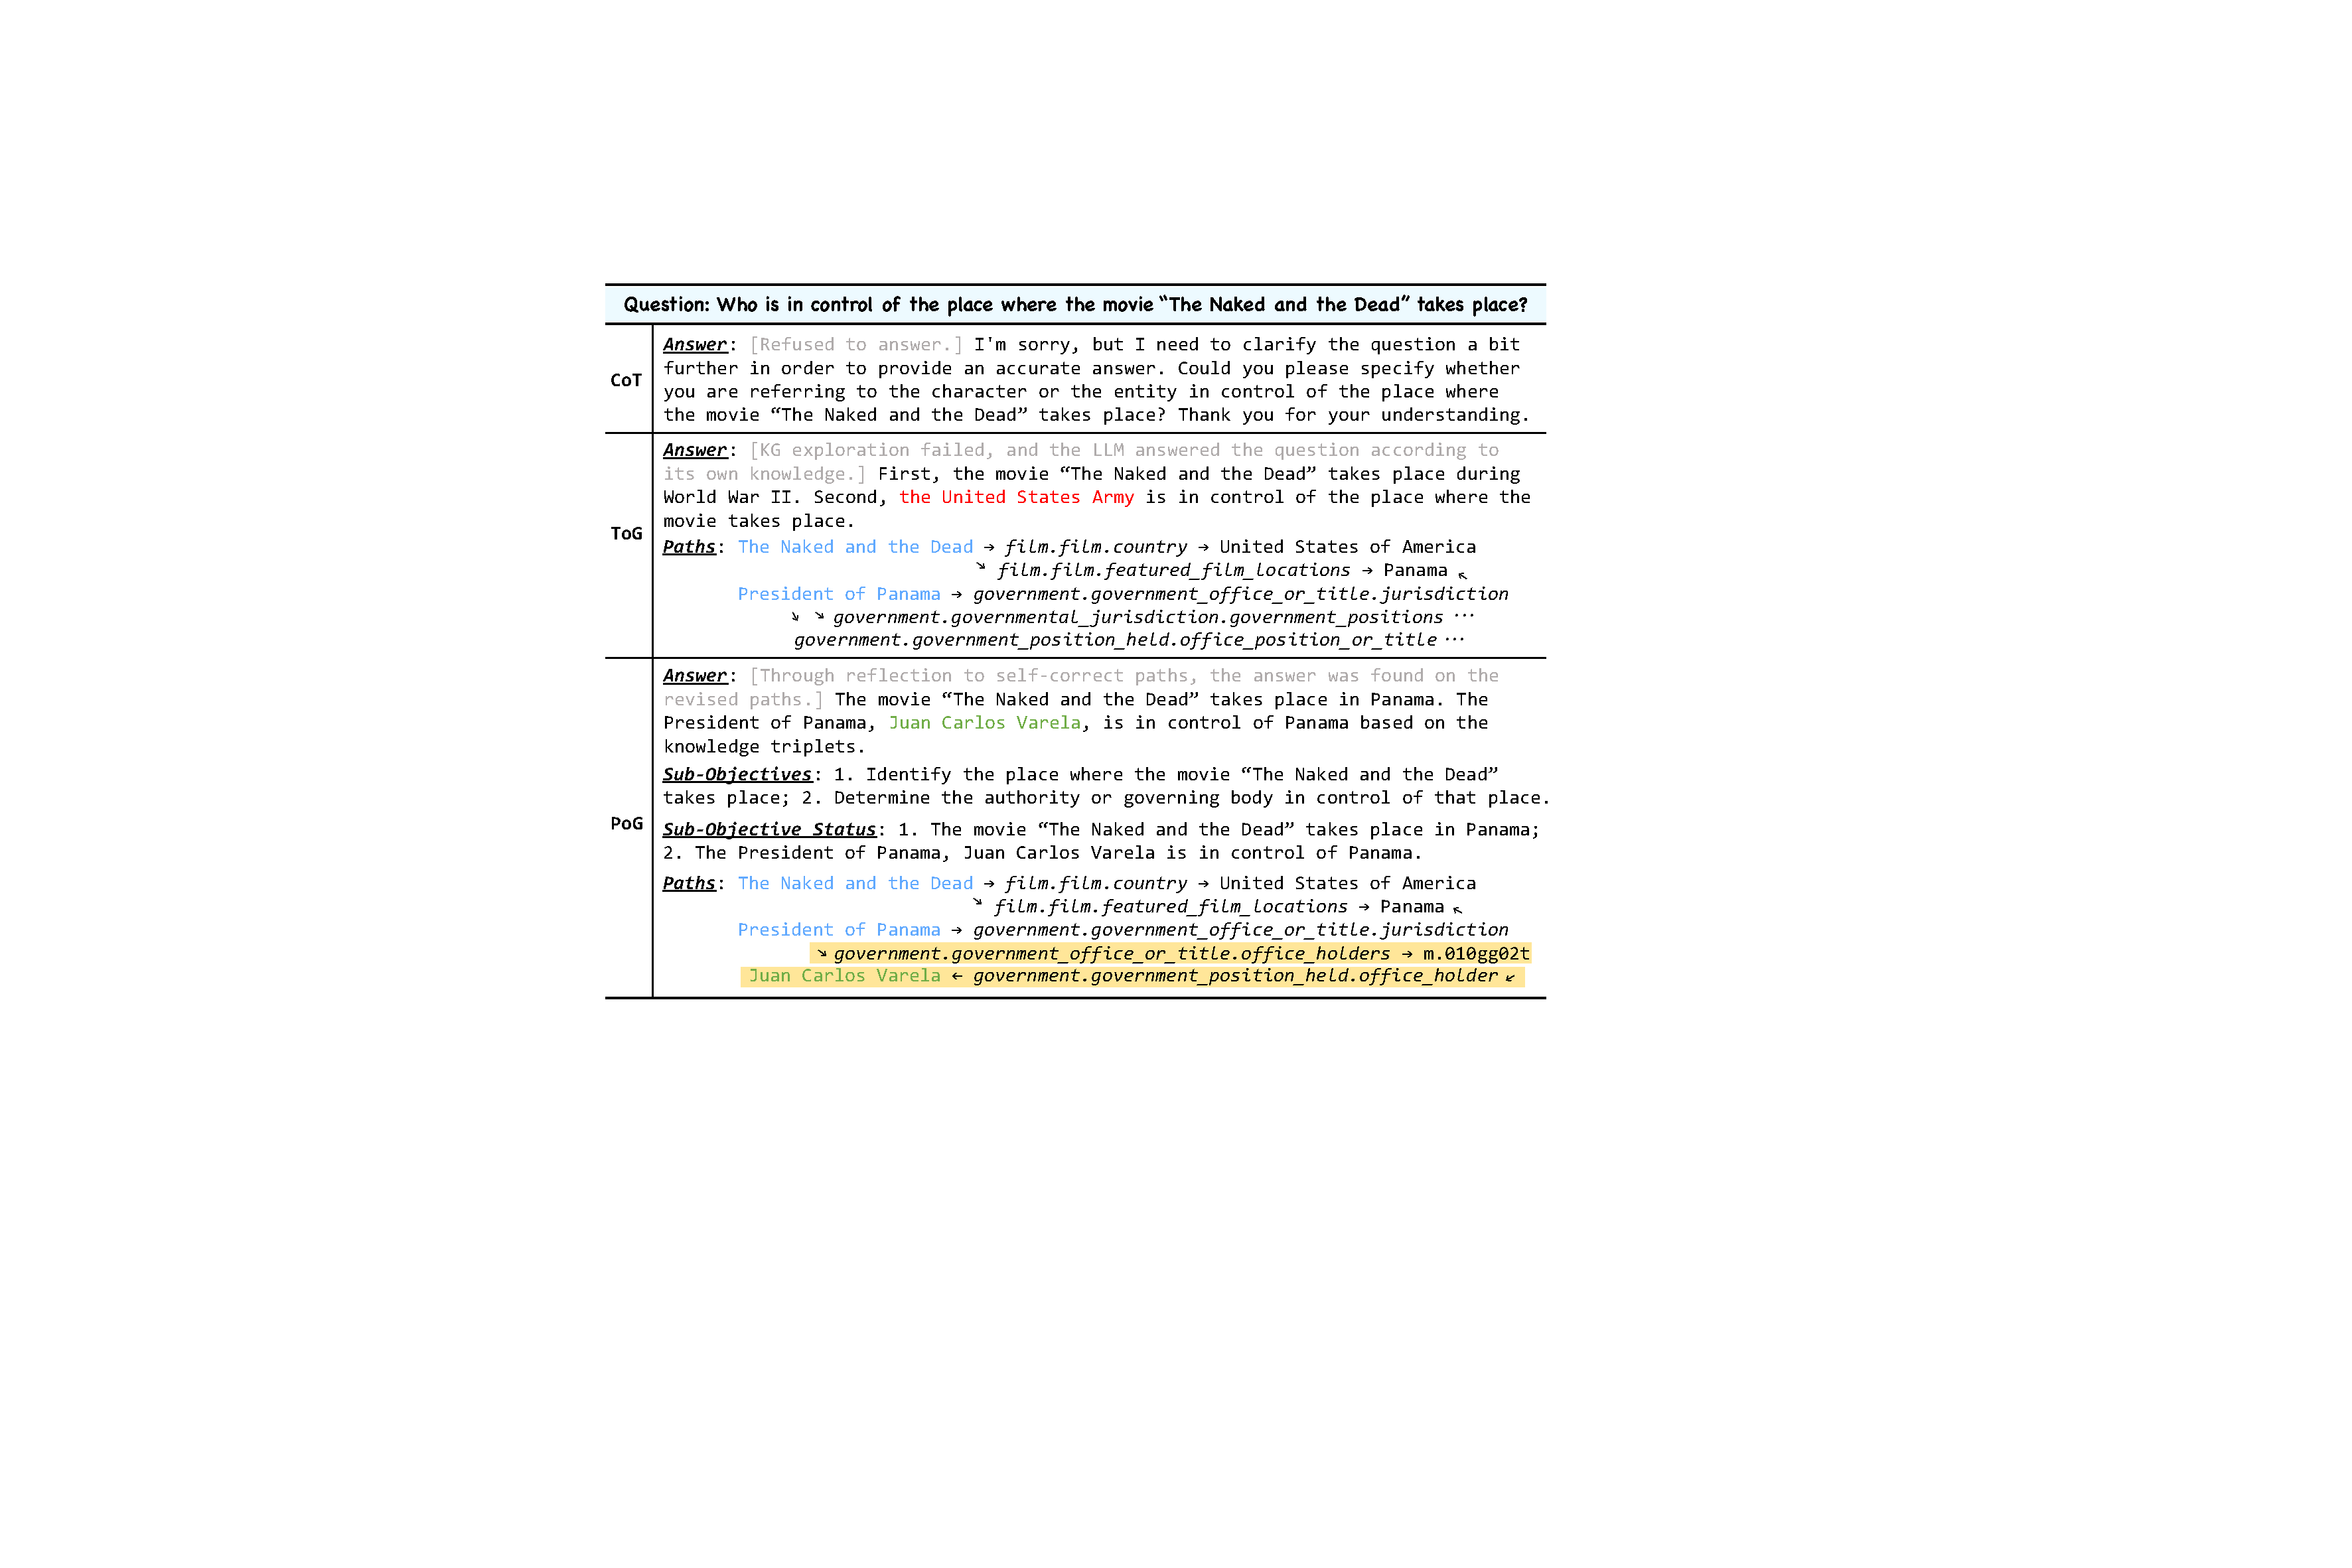
\includegraphics[width=\linewidth]{case-cly.pdf}
 % \vspace{-4mm}
        \setlength{\abovecaptionskip}{-2mm}
        \setlength{\belowcaptionskip}{-2mm}
	\caption{A typical case to compare different methods to answer the complex question. 
 For the convenience of display, we only provide the sub-objective status and partial reasoning paths stored in memory.
 Topic entities, wrong answers, and correct answers are highlighted in blue, red, and green. The revised path is highlighted with a yellow background.}
        % \vspace{-3mm}
	\label{Fig:case}
\end{figure*}
Figure~\ref{Fig:case} shows a typical case from the testing results on CWQ dataset. We compare the results of PoG, ToG, and CoT in answering the question ``Who is in control of the place where the movie `The Naked and the Dead' takes place?''. The underlying LLMs they used are all based on GPT-3.5.
PoG initially identifies a flexible number of relations related to the topic entities. Specifically, for ``The Naked and the Dead'', PoG successfully discovers that the movie takes place in Panama, while for ``President of Panama'', the LLM thinks that only the relation ``government.government\_office\_or\_title.jurisdiction'' is relevant. Upon retrieval, no information is found regarding the person in control of Panama. 
This triggers reflection as PoG realizes that it lacks sufficient information.
With the memory, PoG refers to the sub-objective status and recognizes that it already knows the movie location (Panama) for sub-objective \#1 but is unaware of the person in control of Panama for sub-objective \#2. 
Based on the current reasoning paths, PoG makes a decision to execute self-correction and returns to exploring the relation not previously explored for ``President of Panama''.
Due to the task decomposition, during the self-correction process, it becomes easier to identify the correct relation ``government.government\_office\_or\_title.office\_holders'' according to the sub-objectives. 
Through the guidance, memory, and reflection mechanisms, PoG successfully finds the correct answer, ``Juan Carlos Varela''.
In contrast, ToG fails to identify the most relevant relation concerning ``President of Panama'' and continues exploring incorrect paths. This consumes a significant amount of time and ultimately leads to an erroneous answer due to the hallucination.
CoT refuses to answer directly since the LLM realizes its lack of knowledge regarding the answer and requires additional information to be provided.
From this analysis, it is evident that PoG outperforms ToG and CoT. PoG successfully leverages sub-objective status to self-correct the exploration path in the reflection stage and finally provides the correct answer. 
% This highlights the significance of PoG's graph-based reasoning approach and its ability to identify and utilize relevant relationships efficiently.

% 我们对比了我们的PoG和已有的ToG和CoT。给定主题实体The Naked and the Dead 和 President of Panama，PoG首先识别不定数量的和主题实体相关的关系。对于The Naked and the Dead，PoG顺利的探索到了电影take place的地点是Panama。另外，LLM认为只有government.government_office_or_title.jurisdiction是和President of Panama比较相关的关系，但是检索后发现并不能找到in control of the place的人，在这时PoG因为没有得到充分的信息触发了反思。具体地，PoG通过memory中的子目标状态中知道已经知道子目标1的电影地点是Panama，还不知道子目标2中in control of Panama的是谁，基于当前的推理路径，做出了执行self-correction的决策，回到President of Panama开始探索之前没探索过的关系。由于子目标的拆分，在self-correct路径的时候能够根据子目标的语义更容易识别到正确的关系government.government_office_or_title.office_holders，从而找到正确的答案Juan Carlos Varela。相比之下，ToG没有判断出和President of Panama最相关的关系，并且在错误的路径上继续了错误的探索。这样不仅消耗了大量的时间，还因为幻觉而回答错误。CoT直接拒绝了回答，因为LLM认为自己不知道这个答案，需要额外的知识提供给LLM。
\vspace{-2mm}
\section{Related Work}
\vspace{-2mm}
% In this section, we present the related work of our paper in two directions, LLM reasoning and KG-augmented LLM.
\noindent \textbf{LLM Reasoning.}
To encourage LLMs to engage in reasoning rather than simply providing answers directly, many researchers instruct LLMs to generate the process of thinking in their outputs~\cite{wei2022chain, kojima2022large, zhou2022least}. 
In the early stages, Chain of Thought (CoT)~\cite{wei2022chain} was designed to provide a few examples of intermediate natural language reasoning steps as the prompt.
% or to solve a specific problem
% 变体，不同的context数量或者不同的思维形式，比如图、树、
After that, several variants of CoT reasoning with different forms like Tree-of-Thought~\cite{yao2024tree}, Graph-of-Thought~\cite{besta2024graph}, Memory of Thought~\cite{li2023mot}, and Skeleton-of-Thought~\cite{ning2023skeleton} were proposed to enhance the thinking process.
% After that, several variants of CoT reasoning in various forms or  were proposed , such as Zero-shot-CoT~\cite{kojima2022large}, least-to-most~\cite{zhou2022least}, complex CoT~\cite{fu2022complexity}, Auto-CoT~\cite{zhang2022automatic}, , . 
% 图上的推理
% 核心思想：通过feedback或reward来判断是否需要纠正，
However, LLMs may make mistakes during the reasoning process.
Hence, many works~\cite{shinn2023reflexion, kim2023prospector, madaan2023self, miao2023selfcheck} designed self-correction mechanisms based on feedback to rectify flawed reasoning and ensure accuracy.
% TODO：修改llm graph引用
Additionally, large efforts were dedicated to guiding LLMs in understanding complex graph structures~\cite{tang2023graphgpt, tan2024musegraph} and improving their graph reasoning across different graph tasks~\cite{chen2024collaboration, chen2022multi, chen2020mmea}.
% For example, GraphGPT~\cite{} explores self-supervised graph structural signals and task-specific graph instructions, to in understanding complex graph structures and improving their adaptability across different downstream task.
% aligns LLMs with graph structural knowledge with a graph instruction tuning paradigm.
However, it is still an open issue to address the outdated knowledge, hallucinations, and opaque decision-making for LLM reasoning.

% \vspace{-2mm}
\noindent \textbf{KG-Augmented LLM.}
% \vspace{-2mm}
Despite the pre-training of LLMs on massive corpora, they still suffer from limitations such as outdated knowledge, hallucinations, and opaque decision-making.
An effective approach to address these limitations is to leverage KGs for explicit and editable knowledge provision to LLMs.
Previous studies integrated KGs into LLM pre-training~\cite{zhang2019ernie, wang2021kepler} or fine-tuning~\cite{yao2019kg, luo2024reasoning} stage, but they merely inject structured knowledge into LLMs' parameters and still leave these limitations unexplored. 
Therefore, several works ~\cite{baek2023knowledge, axelsson2023using,wang2023boosting} first retrieved information from KGs and then directly fed explicit knowledge into LLMs. In this way, LLMs do not involve the graph reasoning process and cannot provide potential insights.
Then, a novel KG-augmented LLM paradigm~\cite{jiang2023structgpt,sun2024think} was proposed to treat the LLM as an agent to interactively explore related entities and relations on KGs and perform reasoning based on the retrieved knowledge.
% KGs and LLMs collaboratively work and complement each other's capabilities in each step of graph reasoning. 
% Some efforts have been made in incorporating KGs into LLM reasoning through explicit and editable knowledge delivery,
% by providing knowledge in an explicit and editable way,
% which can be grouped into semantic parsing~\cite{li2023few, ye2022rng} and retrieval-augmented~\cite{baek2023knowledge, axelsson2023using} methods. 
% However, these methods heavily rely on the LLMs' comprehension of the question or factual evidence from KGs, lacking a comprehensive integration of LLMs and KGs during the reasoning process over the graph.
% They excessively rely on the LLMs’ understanding of the question or factual evidence from KGs, lacks a deep integration of LLMs and KGs during the reasoning process on the graph. 
% Subsequently, a tight-coupling KG-augmented LLM paradigm that integrates LLMs' reasoning into the retrieval process on KGs has been proposed~\cite{sun2024think, luo2024reasoning, wen2023mindmap}.
Although this KG-augmented LLM paradigm has achieved impressive performance, it still faces the challenges of adaptively exploring the KG based on question semantics and self-correcting erroneous reasoning paths.
To the best of our knowledge, our work stands out as a pioneering effort in successfully integrating a reflection mechanism for self-correction and adaptive KG exploration into KG-augmented LLMs, effectively enhancing the LLM's reasoning ability.
% GraphLLM takes a unified, end-to-end approach
% to integrate graph learning models and LLMs, enhancing the overall efficiency by synergizing the strengths of both within a single, cohesive system

% cannot adaptively explore the retrieval space based on the question semantics or self-correct when the reasoning path is wrong.

 % Subsequently, an integrated KG-augmented LLM paradigm was proposed, where LLMs' reasoning is tightly coupled with the retrieval process on KGs~\cite{sun2024think, luo2024reasoning, wen2023mindmap}. Despite achieving impressive performance, this tightly integrated KG-augmented LLM paradigm still faces the challenges of adaptively exploring the retrieval space based on question semantics and self-correction when the reasoning path is incorrect.
% Recent efforts have focused on harnessing the power of KGs to enhance LLMs in two main directions: integrating KGs into LLM pre-training, and injecting KGs into LLM inference.
% Early works mainly integrate KGs into LLM pre-training or fine-tuning stage~\cite{luo2024reasoning}.
% However, these methods only compress structured knowledge into LLM's parameters and do not address the flexibility, reliability, and transparency of LLMs.
% Many works designed knowledge-aware training objectives by incorporating KGs into the training data or leveraging KG prediction tasks as additional supervision.

% For injecting KGs into LLM inference, early efforts focused on fusing KG triples into LLM inputs using attention mechanisms or employing graph encoders to process KG inputs. Subsequent research extended these approaches by incorporating graph neural networks for joint reasoning or introducing interactions between text tokens and KG entities in intermediate layers of LLMs. More recently, the research paradigm has shifted towards prompting fixed pre-trained LLMs with graphical inputs. This line of research includes prompting LLMs for KG entity linking prediction, graph mining, and KG question answering. However, these approaches mostly focus on LLMs' ability to understand graph inputs and either target KG-specific tasks or retrieve and translate facts without considering the structure of the KG.



% 没有自我纠正的图推理
% In our work, we propose a new self-correction mechanism for LLM's reasoning on graphs.

% For ensuring the model accuracy, self-correct methods have emerged to further improve the reasoning of LLM like Reflexion~\cite{shinn2023reflexion}, ART~\cite{shridhar2023art}, Prospector~\cite{kim2023prospector},
% VTG~\cite{sun2023towards}, Self-Refine~\cite{madaan2023self}, and SelfCheck~\cite{miao2023selfcheck}. 
% 一句话说明和我们的区别，我们提出了一个
% However, their efficacy
% is undermined by undesired and inconsistent
% behaviors, including hallucination, unfaithful reasoning, and toxic content. A promising approach to rectify these flaws is self-correction
% 现在有一些方法对这些reasoning进行了改进，比如self-correct、reflection
% For instance, Zero-shot-CoT~\cite{kojima2022large} is simply prompted to think step by step without any few-shot demonstrations.

% In order to elicit reasoning 

\vspace{-2mm}
\section{Conclusion}
\vspace{-2mm}
In this paper, we proposed a novel self-correcting adaptive planning paradigm for KG-augmented LLM named Plan-on-Graph (PoG).
To the best of our knowledge, we were the first to incorporate a reflection mechanism for self-correction and adaptive KG exploration into KG-augmented LLMs, effectively augmenting LLM's reasoning ability and efficiency.
% which explored the KG efficiently by adapting the breadth according to the semantics of the question and ensured effectiveness through self-correction mechanisms.
PoG first decomposed the question into several sub-objectives, and then repeated the process of exploring reasoning paths, updating memory, and reflecting on the need to self-correct reasoning paths until arriving at the answer.
To be specific, three important mechanisms were designed to work together to guarantee the adaptive breadth of self-correcting planning for graph reasoning, i.e., Guidance, Memory, and Reflection.
Finally, extensive experiments on three real-world KGQA datasets validated not only the effectiveness but also the efficiency of the proposed PoG.

\vspace{-2mm}
\begin{ack}
\vspace{-2mm}
This work was supported in part by the National Key Research and Development Program of China (Grant No. 2023YFF0725001), the National Natural Science Foundation of China (Grant No. 92370204, 62306255), the Guangdong Basic and Applied Basic Research Foundation (Grant No. 2023B1515120057, 2024A1515011839), the Guangzhou-HKUST (GZ) Joint Funding Program (Grant No. 2023A03J0008), and the Alibaba Research Intern Program.
\end{ack}

\bibliographystyle{plain}
\bibliography{main}



\newpage
\appendix

%%%%%%%%%%%%%%%%%%%%%%%%%%%%%%%%%%%%%%%%%%%%%%%%%%%%%%%%%%%%

\appendix
\section*{Appendix}
\setcounter{section}{0}
\renewcommand\thesection{\Alph{section}}
\section{Prompts}

Here, we provide all the prompts used in PoG. To facilitate the LLM output parsing, we require the LLM to provide answers using specific data structures, such as lists and JSON.
Besides, we require the LLM not to output any other irrelevant information to the results. The specific in-context few-shot is shown in code files.
\subsection{Task Decomposition}
\label{prompt:td}

\lstset{
    basicstyle=\ttfamily\small,
    breaklines=true,
    breakindent=0pt,
    % postbreak=\mbox{\textcolor{red}{$\hookrightarrow$}\space},
    breakatwhitespace=false,
    keepspaces=false,
    columns=flexible,
    frame=single,
    framesep=2pt,
    rulecolor=\color{black},
    backgroundcolor=\color{white},
    tabsize=2,
    showstringspaces=false,
    showtabs=false,
    captionpos=b,
    escapeinside={(*@}{@*)}
}

\begin{lstlisting}[language=]
Please break down the process of answering the question into as few sub-objectives as possible based on semantic analysis.

(*@\textit{\texttt{In-Context Few-Shot}}@*)

Now you need to directly output sub-objectives of the following question in list format without other information or notes. 
Q: {}
\end{lstlisting}

% \begin{verbatim}
% Please break down the process of answering the question into as few sub-objectives as possible based on semantic analysis.

% \textsc{In-Context Few-Shot}

% Q: \{\}
\subsection{Path Exploration}
\subsubsection{Relation Exploration }
\label{prompt:re}
\begin{lstlisting}[language=]
Please provide as few highly relevant relations as possible to the question and its sub-objectives from the following relations (separated by semicolons).

(*@\textit{\texttt{In-Context Few-Shot}}@*)

Now you need to directly output relations highly related to the following question and its sub-objectives in list format without other information or notes.
Q: {}
Sub-Objectives: {}
Topic Entity: {}
Relations: {}
\end{lstlisting}
\subsubsection{Entity Exploration}
\label{prompt:ee}
\begin{lstlisting}[language=]
Which entities in the following list ([] in Triples) can be used to answer the question? Please provide the minimum possible number of entities, and strictly adhering to the constraints mentioned in the question. 

(*@\textit{\texttt{In-Context Few-Shot}}@*)

Now you need to directly output the entities from [] in Triplets for the following question in list format without other information or notes.
Q: {}
Triplets: {}
\end{lstlisting}
\subsection{Memory Updating}
\label{prompt:mu}
\begin{lstlisting}[language=]
Based on the provided information (which may have missing parts and require further retrieval) and your own knowledge, output the currently known information required to achieve the sub-objectives.

(*@\textit{\texttt{In-Context Few-Shot}}@*)

Now you need to directly output the results of the following question in JSON format without other information or notes. 
Q: {}
Sub-Objectives: {}
Memory: {}
Knowledge Triplets: {}
\end{lstlisting}
\subsection{Evaluation}
\subsubsection{Answer Question}
\label{prompt:aq}
\begin{lstlisting}[language=]
Please answer the question based on the memory, related knowledge triplets and your knowledge.

(*@\textit{\texttt{In-Context Few-Shot}}@*)

Now you need to directly output the results of the following question in JSON format (must include "A" and "R") without other information or notes. If the triplets explicitly contain the answer to the question, prioritize the fact of the triplet over memory.
Q: {}
Memory: {}
Knowledge Triplets: {}
\end{lstlisting}
\subsubsection{Reflection}
\label{prompt:reflection}
\begin{lstlisting}[language=]
Based on the current set of entities to be retrieved and the known information including memory and triplets, is it necessary to add additional entities for answering the question?

(*@\textit{\texttt{In-Context Few-Shot}}@*)

Now you need to directly output the results of the following question in the JSON format (must include "Add" and "Reason") without other information or notes.
Q: {}
Entities set to be retrieved: {}
Memory: {}
Knowledge Triplets: {}

\end{lstlisting}

\begin{lstlisting}[language=]
Please select the fewest necessary entities to be retrieved for answering the Q from Candidate Entities, based on the current known information (Memory), the reason for additional retrieval, and your own knowledge.

(*@\textit{\texttt{In-Context Few-Shot}}@*)

Now you need to directly output the results for the following Q in the list format without other information or notes.
Q: {}
Reason: {}
Candidate Entities: {}
Memory: {}

\end{lstlisting}
% \begin{lstlisting}[language=SPARQL, caption={Example SPARQL query}, label=lst:sparql_query]
% PREFIX rdfs: <http://www.w3.org/2000/01/rdf-schema#>
% SELECT ?subject ?label
% WHERE {
%   ?subject rdfs:label ?label
% }
\lstdefinestyle{mystyle}{
    backgroundcolor=\color{gray!3},
    basicstyle=\footnotesize\ttfamily,
    breaklines=true,
    keywordstyle=\color{blue},
    morekeywords={PREFIX, SELECT, WHERE, FILTER, LIMIT, OFFSET}
}
\section{Search SPARQL}
\label{Apx:sparql}
To automatically process the KG data in PoG, we pre-define the SPARQL for Freebase queries, which can be executed by filling in the entity's mid and relation.
\subsection{Relation Search}
\label{Apx:queryrel}

\begin{lstlisting}[language=SPARQL,style=mystyle]
PREFIX ns: <http://rdf.freebase.com/ns/>
SELECT DISTINCT ?relation
WHERE {
  ns:mid ?relation ?x .
}
\end{lstlisting}

\begin{lstlisting}[language=SPARQL,style=mystyle]
PREFIX ns: <http://rdf.freebase.com/ns/>
SELECT DISTINCT ?relation
WHERE {
  ?x ?relation ns:mid .
}
\end{lstlisting}
% PREFIX ns: <http://rdf.freebase.com/ns/>\\
% SELECT DISTINCT ?relation\\
% WHERE \{\\
% \hspace*{0.5cm} ns:mid ?relation ?x .\\
% \}
% \\


% PREFIX ns: <http://rdf.freebase.com/ns/>\\
% SELECT DISTINCT ?relation\\
% WHERE \{\\
% \hspace*{0.5cm}   ?x ?relation ns:mid .\\
% \}
\subsection{Entity Search}
\label{Apx:queryent}
\begin{lstlisting}[language=SPARQL,style=mystyle]
PREFIX ns: <http://rdf.freebase.com/ns/>
SELECT ?tailEntity
WHERE {
  ns:mid ns:relation ?tailEntity .
}
\end{lstlisting}
\begin{lstlisting}[language=SPARQL,style=mystyle]
PREFIX ns: <http://rdf.freebase.com/ns/>
SELECT ?tailEntity
WHERE {
  ?tailEntity ns:relation ns:mid .
}

\end{lstlisting}
% PREFIX ns: <http://rdf.freebase.com/ns/>\\
% SELECT ?tailEntity\\
% WHERE \{\\
% \hspace*{0.5cm} ns:mid ns:relation ?tailEntity .\\
% \}
% \\


% PREFIX ns: <http://rdf.freebase.com/ns/>\\
% SELECT ?tailEntity\\
% WHERE \{\\
% \hspace*{0.5cm} ?tailEntity ns:relation ns:mid  .\\
% \}

\subsection{Entity Name Search}
\begin{lstlisting}[language=SPARQL,style=mystyle, escapechar=|]
PREFIX ns: <http://rdf.freebase.com/ns/>
SELECT DISTINCT ?tailEntity
WHERE {
  {
    ?entity ns:type.object.name ?tailEntity .
    FILTER(?entity = ns:mid)
  }
  UNION
  {
    ?entity <http://www.w3.org/2002/07/owl|\#|sameAs> ?tailEntity .
    FILTER(?entity = ns:mid)
  }
}
\end{lstlisting}



% PREFIX ns: <http://rdf.freebase.com/ns/>\\
% SELECT DISTINCT ?tailEntity\\
% WHERE \{\\
%   \{\\
% \hspace*{0.5cm}     ?entity ns:type.object.name ?tailEntity .\\
%  \hspace*{0.5cm}    FILTER(?entity = ns:mid)\\
%   \}\\
%   UNION\\
%   \{\\
%  \hspace*{0.5cm}    ?entity <http://www.w3.org/2002/07/owl\#sameAs> ?tailEntity .\\
% \hspace*{0.5cm}    FILTER(?entity = ns:mid)\\
%   \}\\
% \}
\section{Datasets}
\label{apx:dataset}
In this paper, we use three complex multi-hop KGQA datasets: ComplexWebQuestions~\cite{talmor2018web}, WebQSP~\cite{yih2016value}, and GrailQA~\cite{gu2021beyond}. The statistics of datasets are shown in Table~\ref{Tab:dataset}.
 % ComplexWebQuestions (CWQ) is a dataset for answering complex questions that require reasoning over multiple web snippets. 
WebQSP contains questions from WebQuestions that are answerable by Freebase. It tests I.I.D. generalization on questions.
ComplexWebQuestions (CWQ) extends WebQSP and encompasses four types of complex questions: conjunction, composition, comparative, and superlative.
% , covering 32,585 entities, 3,720 relations across 86 domains
GrailQA is a diverse KGQA dataset built on Freebase, and is designed to test three levels of generalization of models: I.I.D., compositional, and zero-shot.
% \begin{table}[ht]
% \centering
% \caption{Statistics of MMKGs in the dataset. (Rel. T.: Relational Triple, Attr. T.: Attribute Triple, E.-I. Pair: Entity-Image Pair, A. E. Pair: Aligned Entity Pair.)}
% 	\resizebox{8.5cm}{!}
% 	{   
% 		\begin{tabular}{c|ccccc} 
% 			\toprule
% 			\textbf{Dataset}&\textbf{Entity}&\textbf{Rel. T.}&\textbf{Attr. T.}&\textbf{E.-I. Pair}&\textbf{A. E. Pair}\\
% 			\midrule  
% 			FB15K&14,951&592,213&29,395&13,444&-\\
% 			DB15K&12,842&89,197&48,080&12,837&12,846\\
% 			YG15K&15,404&122,886&23,532&11,194&11,199\\
% 			\bottomrule
% 		\end{tabular}
% 	}
% 	\label{Tab:dataset}
% \end{table}
\begin{table}[ht]
\centering
\caption{Statistics of KGQA datasets.}
\begin{tabular}{lcccc} 
    \toprule
    \textbf{Dataset} & \textbf{Answer Format} & \textbf{Train} & \textbf{Test} & \textbf{Licence}\\
    \midrule  
     ComplexWebQuestions & Entity & 27,734 & 3,531& - \\
     WebQSP & Entity/Number & 3,098 & 1,639 & CC Licence \\
     GrailQA & Entity/Number & 44,337 & 1,000 & - \\
    \bottomrule
\end{tabular}
\label{Tab:dataset}
\end{table}

\section{Baseline Descriptions}
\label{Apd:baseline}
The baselines we compare can be categorized into two groups: (1) LLM-only methods;
(2) KG-augmented LLM methods, including fine-tuned and prompting methods. 

\noindent \textbf{LLM-Only Methods}
\begin{itemize}[leftmargin=1cm] 
    \item Standard prompting (IO prompt)~\cite{brown2020language} verifies the ability of LLMs to achieve better performance in task-agnostic, few-shot problems than traditional LMs.
    \item Chain-of-Thought prompting (CoT)~\cite{wei2022chain} generates a series of intermediate reasoning steps in prompts to help LLMs perform better in several NLP tasks.
    \item Self-Consistency (SC)~\cite{wang2023self} samples multiple, diverse reasoning paths through few-shot CoT, and uses the generations to select the most consistent answer. 
    % This helps to boost the performance of CoT prompting on tasks involving arithmetic and commonsense reasoning.
\end{itemize}

% \noindent \textbf{KG-Augmented LLM Methods}

% For CWQ and WebQSP, we select UniKGQA~\cite{jiang2023unikgqa}, TIARA~\cite{shu2022tiara}, RE-KBQA~\cite{cao2023pay}, DeCAF~\cite{yu2023decaf}, and RoG~\cite{luo2024reasoning} as the fine-tuned baselines and KD-CoT~\cite{wang2023knowledge}, KB-BINDER~\cite{li2023few}, StructGPT~\cite{jiang2023structgpt}, Interactive KBQA~\cite{xiong2024interactive}, and ToG~\cite{sun2024think} as the prompting baselines. 

\noindent \textbf{Finetuned KG-Augmented LLM Methods}
\begin{itemize} [leftmargin=1cm] 
    \item UniKGQA~\cite{jiang2023unikgqa} unifies the graph retrieval and reasoning process into a single model with LLMs.
    \item TIARA~\cite{shu2022tiara} first uses BERT to retrieve a set of schema items, which are further used as the input, together with the question, to T5 for plan generation. They also apply constrained decoding but only for grammaticality.
    \item RE-KBQA~\cite{cao2023pay} capitalizes relations in KGs to enhance entity representations and introduce additional supervision to improve the selection of reasoning paths.
    \item DeCAF~\cite{yu2023decaf} combines semantic parsing and LLMs reasoning to jointly generate answers, which also reach salient performance on KGQA tasks.
    \item RoG~\cite{luo2024reasoning} collaborates LLMs with KGs to achieve trustworthy reasoning to leverage structural information.
    \item RnG-KBQA~\cite{ye2022rng} first uses BERT to rank a set of enumerated candidate programs (up to a limited complexity), and then uses T5 to edit the top programs into more complex programs.
    \item FC-KBQA~\cite{zhang2023fc} proposes a fine-to-coarse composition framework to avoid knowledge entanglement and guarantee both generalization ability and logical interpretability. 
    \item Pangu~\cite{gu2023don} considers leveraging the discriminative ability of LLMs. It consists of a symbolic agent with a cooperative neural LLM.
    \item FlexKBQA~\cite{li2024flexkbqa} is a flexible KGQA framework with LLMs. It can utilize a limited set of annotated data to build KGQA for different KGs and query languages.
    \item GAIN~\cite{shu2024distribution} pays attention to the robustness of KGQA models. It proposes a data augmentation method to alleviate this problem and further evaluates the distribution shifts including from different aspects.
\end{itemize}

\noindent \textbf{Prompting KG-Augmented LLM Methods}
\begin{itemize}[leftmargin=1cm] 
    \item KB-BINDER~\cite{li2023few} is developed to challenge the heterogeneity of items from different KGs. It enables few-shot in-context learning over KGQA tasks.
    % is the first method that
    \item KD-CoT~\cite{wang2023knowledge} retrieves relevant knowledge from KGs to generate faithful reasoning plans for LLMs.
    \item 
    StructGPT~\cite{jiang2023structgpt} defines the interface of KG data to implement knowledge access and filtering with finite quantity, and leverage the LLM to infer the answer or subsequent planning repeatedly.

    \item Interactive KBQA~\cite{xiong2024interactive} interacts with KGs directly and then generates logical forms. The interactions are under three designed universal APIs for KGs.
    \item ToG~\cite{sun2024think} iteratively retrieves relevant triplets from KGs and employs the LLM to assess whether the reasoning paths in beam search are sufficient for answering the question and if further retrieval of the next hop is necessary.
\end{itemize}

\section{Implementation Details} 
\label{modelset}
In our experiments, we use GPT-3.5 and GPT-4 to serve as the underlying LLMs. We call them by the OpenAI official API~\footnote{\url{https://platform.openai.com/docs/api-reference.}}.
We set the temperature parameter to 0.3, frequency penalty to 0, and presence penalty to 0.
The maximum token length for generation is 1024. In all experiments, the depth of exploration is set to 4 to avoid endless exploration.
The experiments are conducted on a server with two 
Intel(R) Xeon(R) CPU E5-2682 v4 @ 2.50GHz and 256 GB RAM memory.
\section{Depth Sensitivity}\begin{wrapfigure}[10]{r}{5.5cm}
	\centering
 \vspace{-1.2cm}
	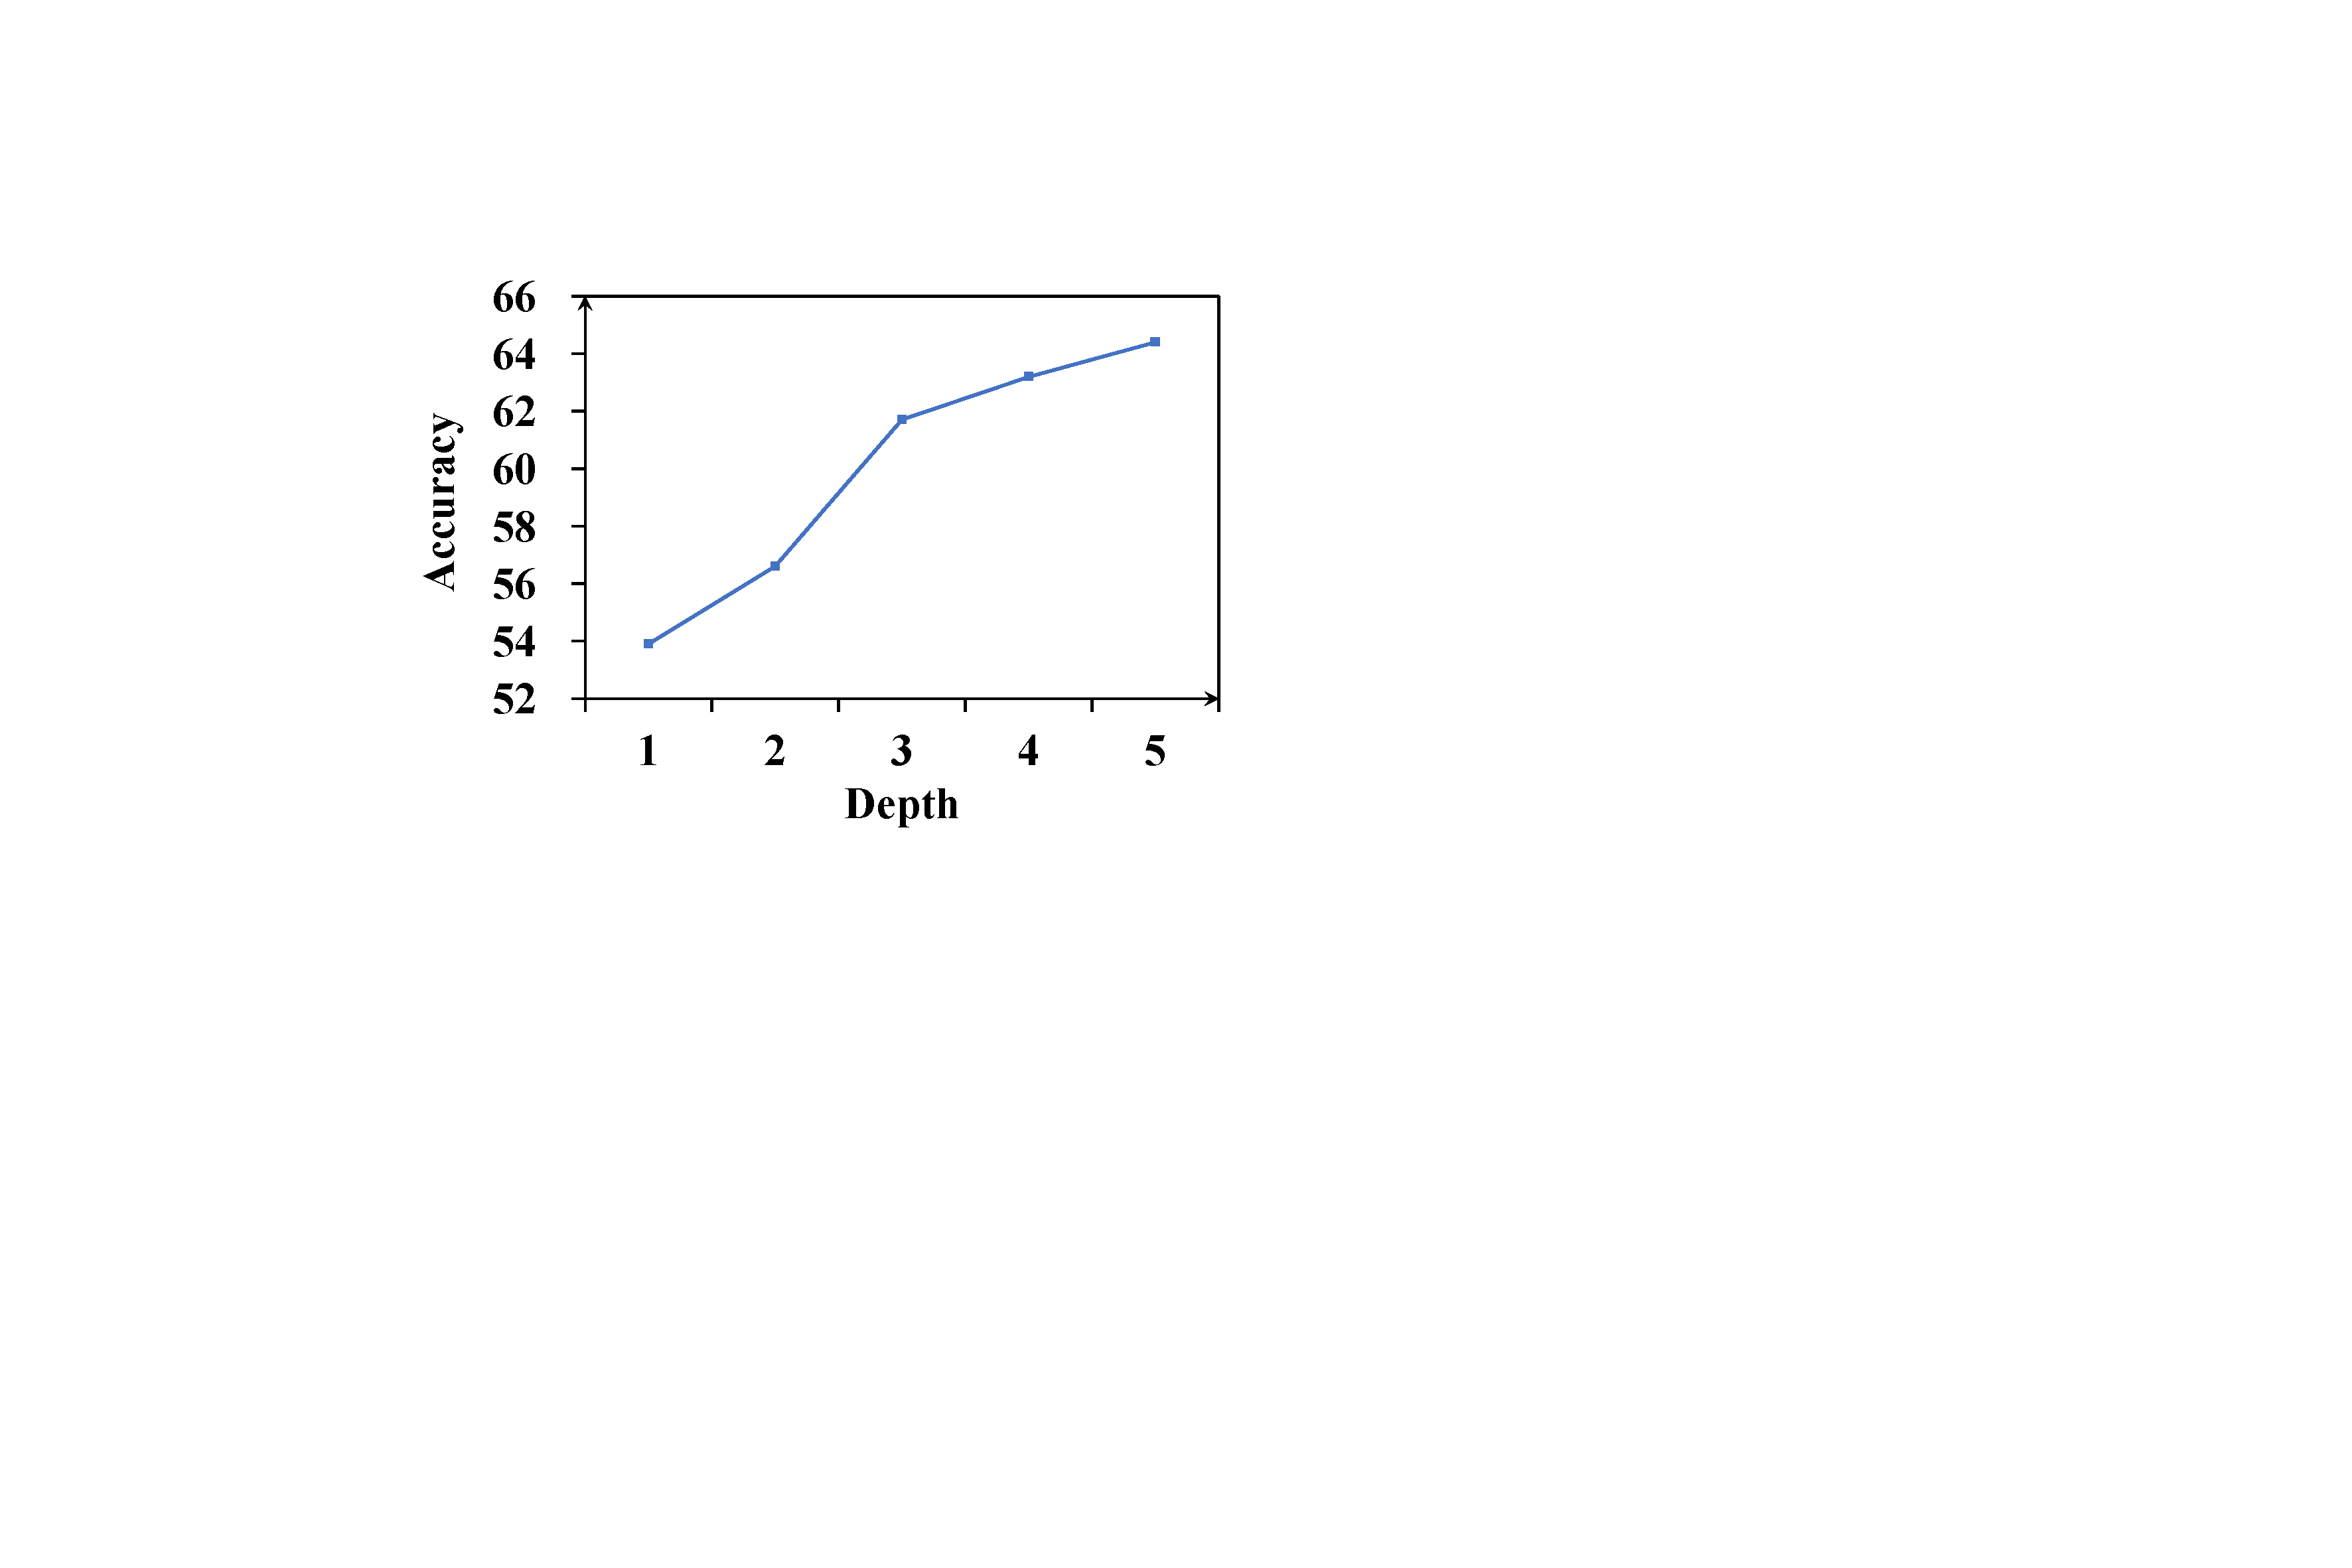
\includegraphics[width=\linewidth]{depth.pdf}
        \setlength{\abovecaptionskip}{-2mm}
        \setlength{\belowcaptionskip}{2mm}
	\caption{The impact of exploration depth on the performance of PoG.}
 % \vspace{-3mm}
	\label{Fig:depth}
\end{wrapfigure}
Since LLMs are not entirely certain about when to stop, we need to manually set the depth of KG exploration to avoid endless exploration.
To investigate the impact of exploration depth on PoG performance, we conduct experiments with depth settings ranging from 1 to 5 on CWQ dataset. As shown in Figure~\ref{Fig:depth}, increasing the depth will improve the performance of PoG. Beyond a depth of 4, the improvement becomes less noticeable. 
The increase in depth leads to exponential growth in resource and time consumption. Considering the balance between efficiency and effectiveness, we set the depth to 4.
% Therefore, we set the depth to 4.


\section{Case Analysis}
\begin{wrapfigure}[13]{r}{4cm}
	\centering
 \vspace{-1.3cm}
	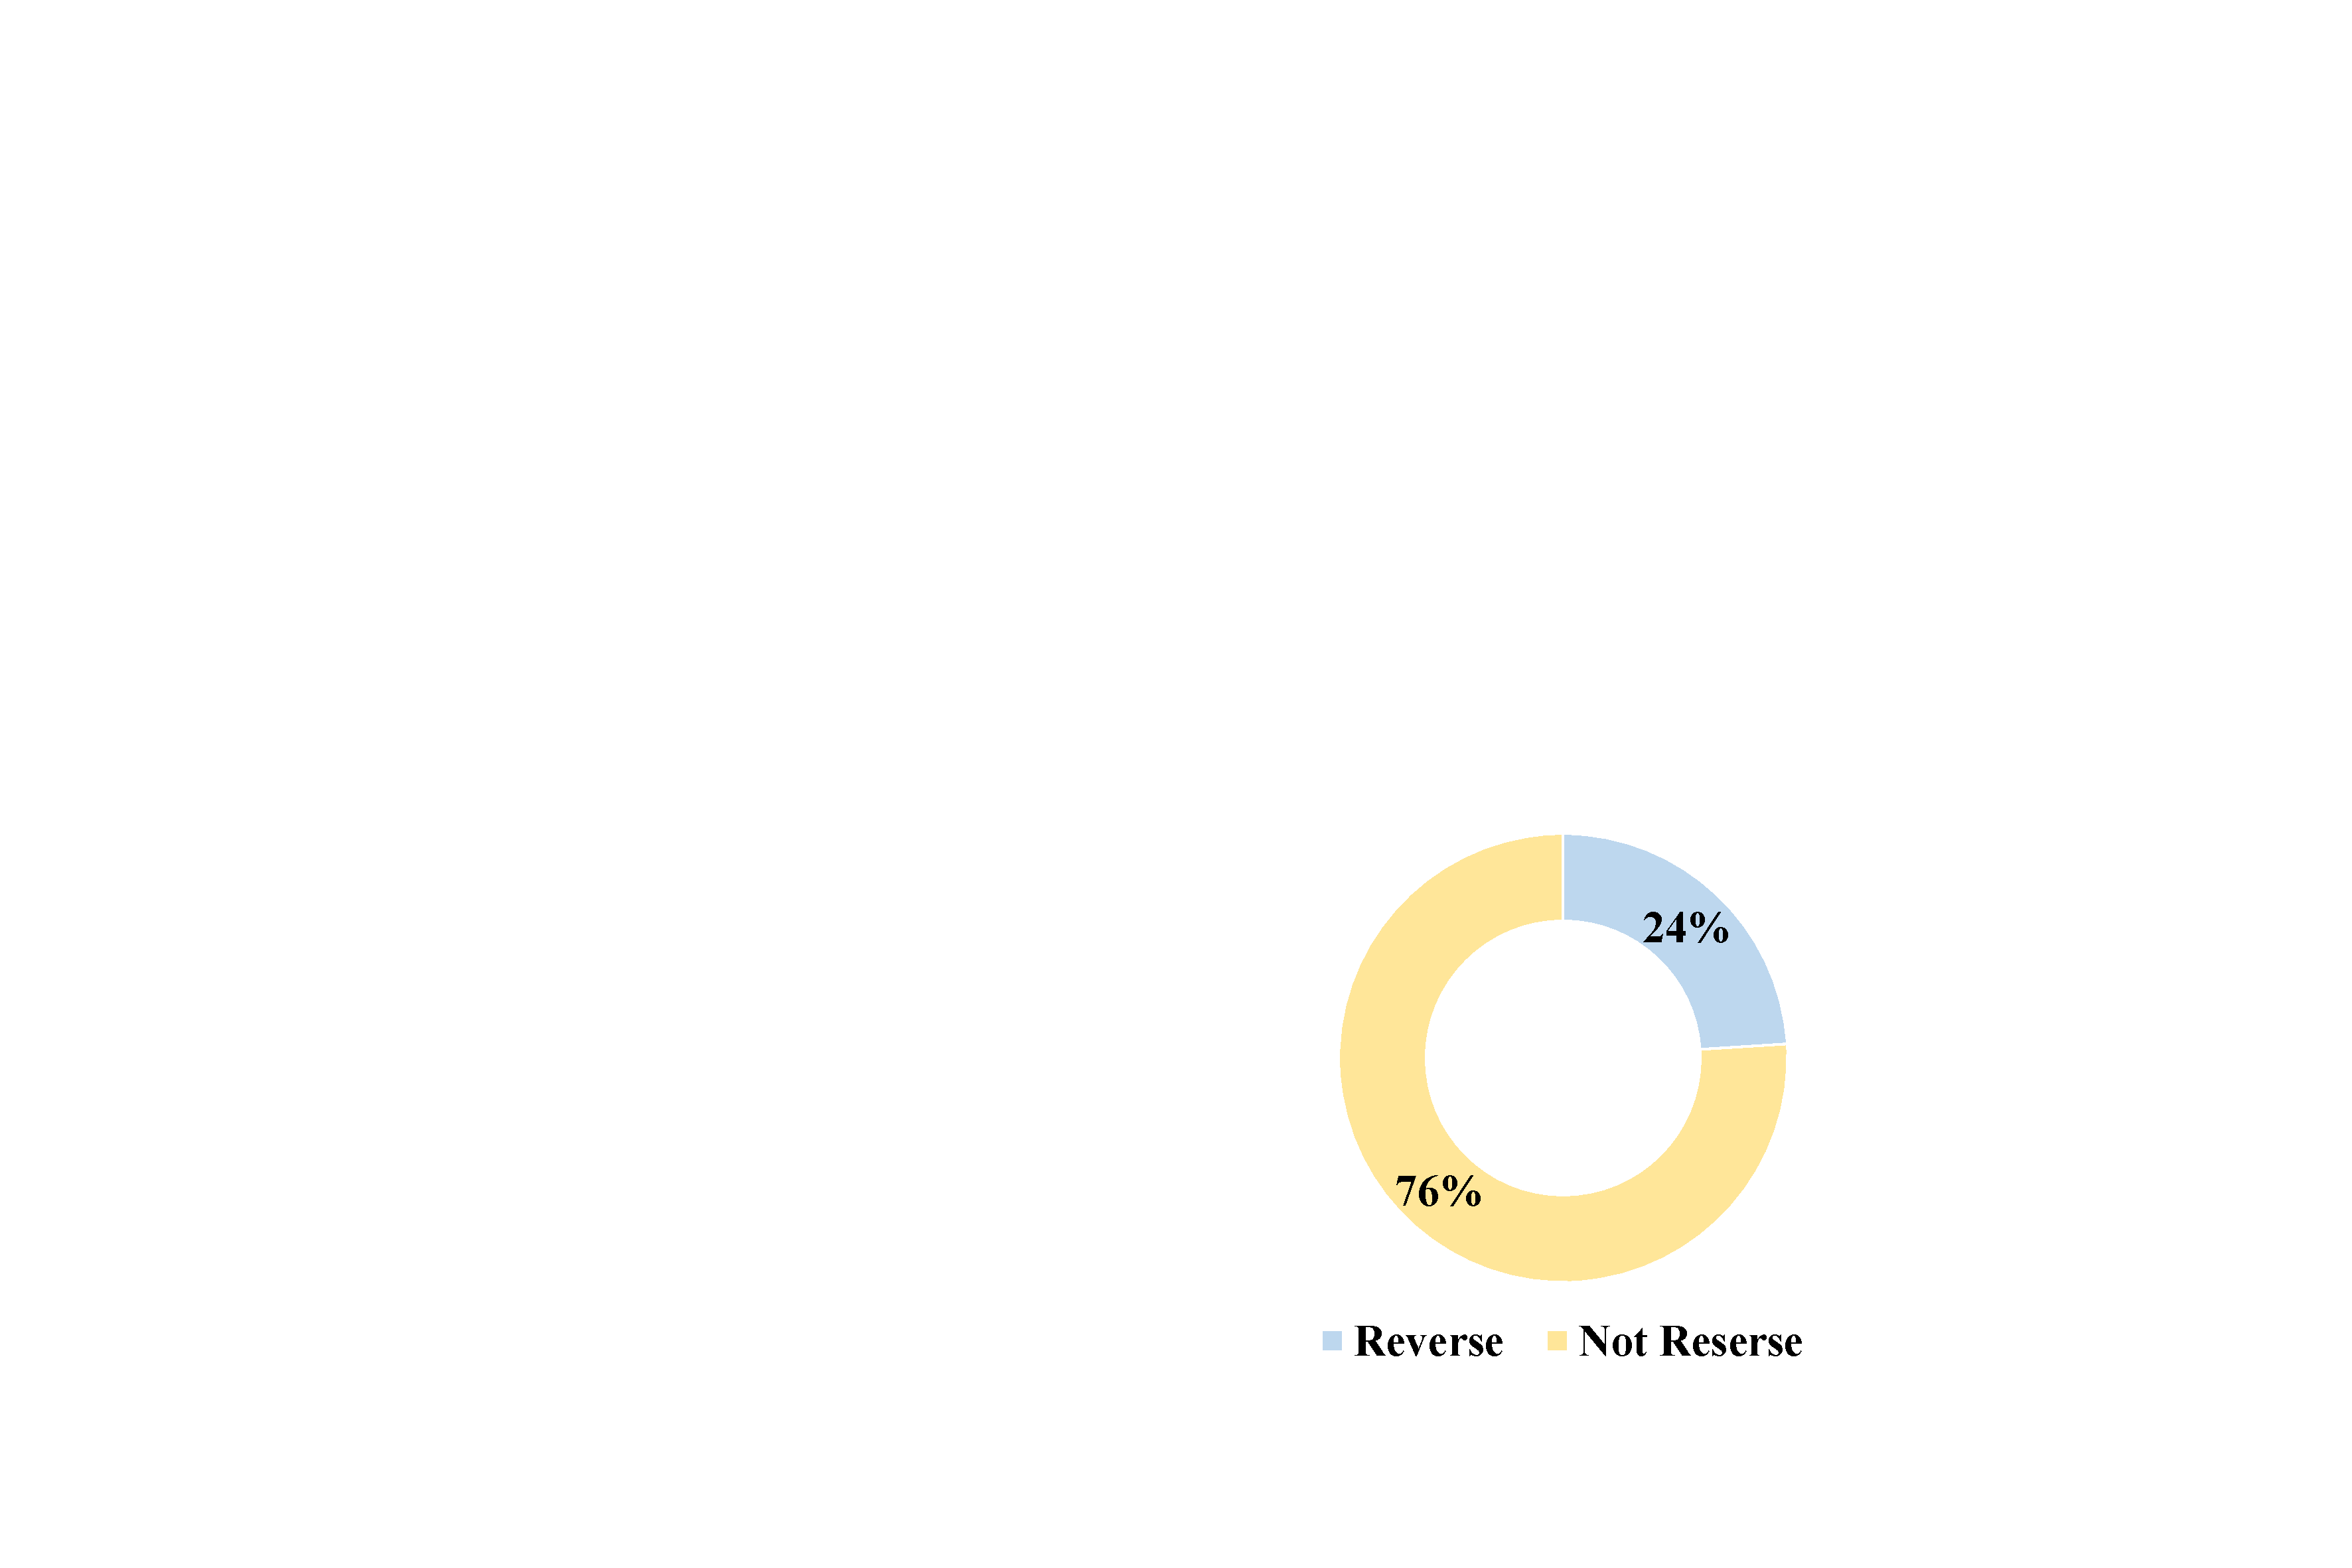
\includegraphics[width=\linewidth]{reverse-ratio.pdf}
 % \vspace{-4cm}
        \setlength{\abovecaptionskip}{-2mm}
        \setlength{\belowcaptionskip}{2mm}
	\caption{The proportion of cases with reverse occurrences among all data.}
 % \vspace{-3mm}
	\label{Fig:reverse_r}
\end{wrapfigure}
In PoG, we design a reflection mechanism to provide the opportunity for self-correction for exploring reasoning paths.
In Figure~\ref{Fig:reverse_r}, we calculate the proportion of cases with reverse occurrences among all questions in CWQ, and the results show that 24\% of cases involve reversing during the exploration process to achieve self-correction. This demonstrates that LLMs are indeed not always capable of making correct judgments in KG exploration and that self-correction is necessary for KG-augmented LLMs.
Figure~\ref{Fig:prop_reverse} presents the proportion of correct answers obtained by PoG after self-correction on three datasets.
Overall, the self-correction in PoG appears to have positively impacted the accuracy of KGQA, particularly for the WebQSP and CWQ datasets, where the proportion of correct answers reached 64\% and 48\% after the self-correction process.
This analysis suggests that the reflection mechanism in PoG has the potential to enhance the reasoning capabilities of KG-augmented LLM and improve the performance across various datasets by allowing for self-correction and exploration of alternative reasoning paths.
\begin{figure*}[h]
	\centering
        % \vspace{-2.8mm}
	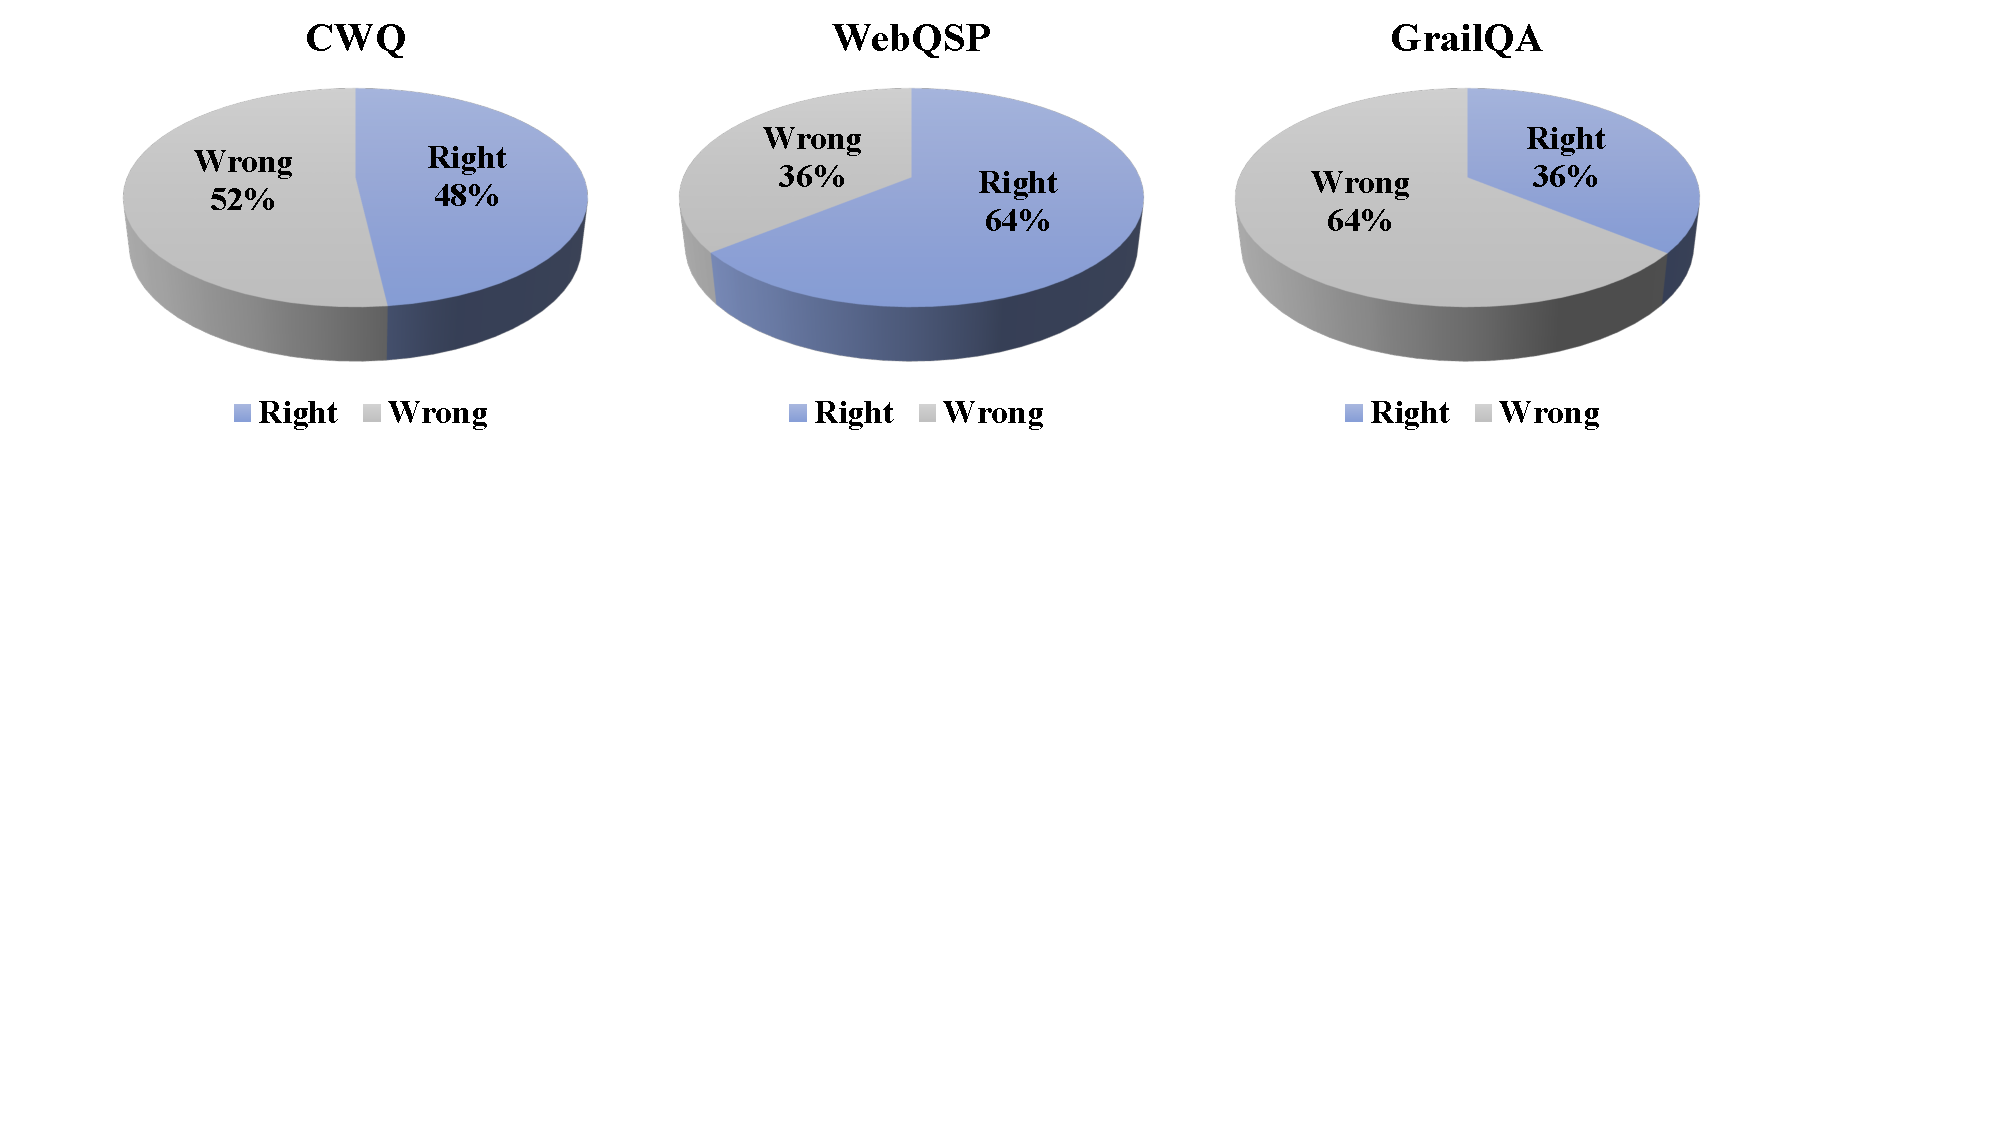
\includegraphics[width=\linewidth]{casestudy-reverse.pdf}
 % \vspace{-4mm}
        \setlength{\abovecaptionskip}{-2mm}
        \setlength{\belowcaptionskip}{-2mm}
	\caption{The proportion of correct answers obtained by PoG after self-correction.}
        % \vspace{-3mm}
	\label{Fig:prop_reverse}
\end{figure*}



% PoG首先自适应地识别出了和主题实体Claude Debussy的和问题最相关的关系music.artist.genre。由于不限定推理路径的广度，PoG将多个候选实体全部判断为和问题相关的。在接下来对主题实体Suzanne Farrell: Elusive Muse的探索中，由于PoG在memory中记录了已知的子目标状态1信息，直接自适应地只选择了Ballet作为推理路径。通过自适应广度和记录子目标的状态，PoG成功且高效的给出了正确答案
% 而ToG在有多个候选实体时，都是随机选取的路径进行探索，这样只找到了子目标一中的条件。最后大模型只记得the genre of music favored by Claude Debussy而遗忘了子目标二中的条件，回答了incidental music.
% CoT直接出现幻觉而乱说了一个不相关的答案impressionism。
Besides, Figure~\ref{Fig:apx-case} shows another typical case from the testing results on CWQ dataset.
We compare the results of PoG, ToG, and CoT in answering the question ``What genre of music favored by Claude Debussy appears in the movie Suzanne Farrell: Elusive Muse?''. 
PoG first adaptively identifies the most relevant relation ``music.artist.genre'' to the topic entity ``Claude Debussy''. 
Without constraining the breadth of reasoning paths, PoG considers multiple candidate entities as potentially relevant to the question. 
In the subsequent exploration of the topic entity ``Suzanne Farrell: Elusive Muse'', PoG adaptively chooses only ``Ballet'' as the relevant entity, as it records the known information of sub-objective \#1 in memory. Through adaptive breadth and memorization of sub-objective status, PoG successfully and efficiently provides the correct answer.
In contrast,  ToG randomly explores paths when faced with multiple candidate entities, only finding one condition from sub-objective \#1. Finally, ToG only remembers the genre of music favored by ``Claude Debussy'' but forgets the condition from sub-objective \#2, answering ``Incidental music''.
 CoT directly hallucinates an irrelevant answer, ``Impressionism''.
 This case indicates the effectiveness of adaptive breadth and memorization of sub-objective status.
 \begin{figure*}[t]
	\centering
        % \vspace{-1mm}
	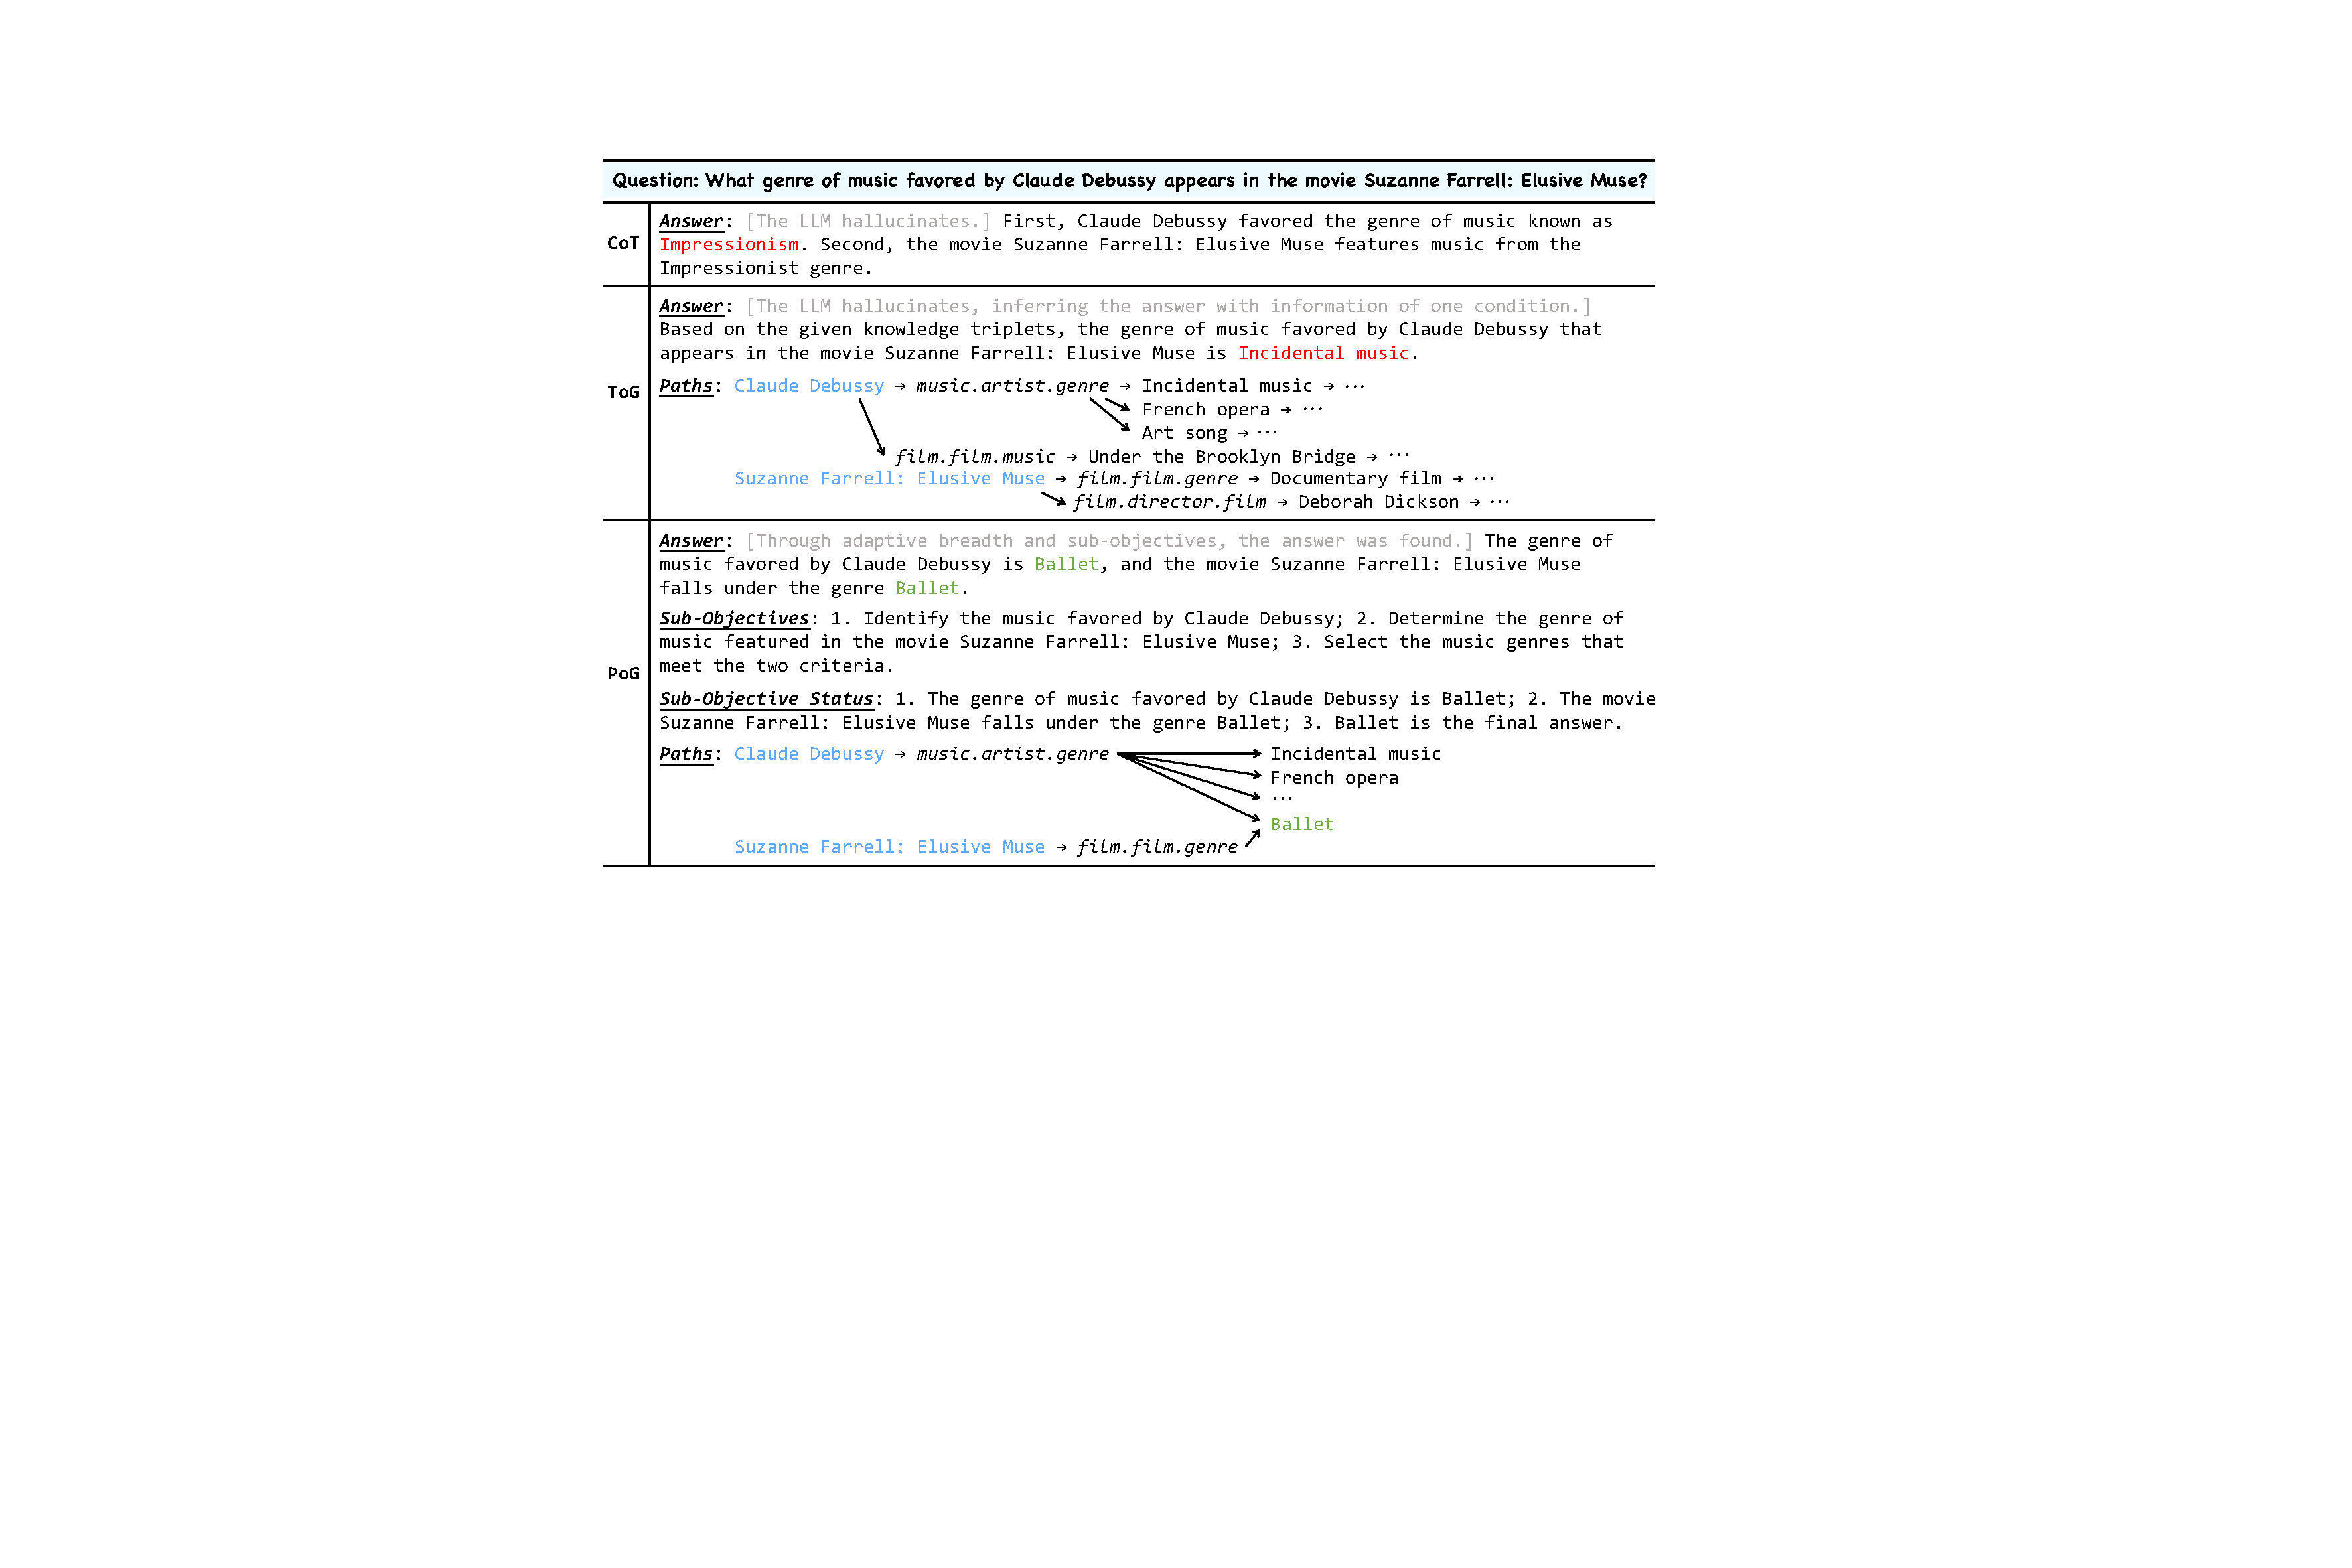
\includegraphics[width=\linewidth]{apd-case-cly.pdf}
 % \vspace{-4mm}
        \setlength{\abovecaptionskip}{-2mm}
        \setlength{\belowcaptionskip}{-4mm}
	\caption{A typical case to compare different methods to answer the complex question. 
 For the convenience of display, we only provide the sub-objective status and partial reasoning paths stored in memory.
 Topic entities, wrong answers, and correct answers are highlighted in blue, red, and green. 
  }
        % \vspace{-3mm}
	\label{Fig:apx-case}
\end{figure*}
\section{Broader Impact \& Limitation}
\label{apdx:lim}
In the current research landscape, PoG carries a significant broader impact, primarily reflected in its enhancement of complex reasoning capabilities for KG-augmented LLM. By innovatively integrating guidance, memory, and reflection mechanisms, PoG not only strengthens the model's flexibility and accuracy when facing complex queries but also enhances its ability to self-correct erroneous reasoning paths. This self-correcting adaptive planning paradigm enables the model to backtrack and adjust reasoning directions when faced with invalid initial assumptions or impasses, resulting in an optimal solution search. Additionally, the broader impact of PoG is manifested in several other aspects: (1) Improving Efficiency and Effectiveness in Problem-Solving: By dynamically adjusting exploration breadth and employing self-correction mechanisms, PoG can more efficiently handle complex questions and provide more accurate answers, significantly enhancing the overall performance of KGQA systems.
(2) Enhancing the Robustness and Adaptability of LLMs: Through its memory mechanism, which records and tracks the completion status and reasoning paths of each sub-objective, PoG enables the LLM to more robustly deal with the uncertainty and complexity of questions, making it more precise and reliable across a wide range of applications.
(3) Fostering Innovation in the Field of Artificial Intelligence: PoG's integration of meta-cognitive capabilities into reasoning and planning processes represents an innovative attempt that could further propel research and innovation in broader AI technologies within the artificial intelligence field.
(4) Improving User Experience and Expanding Application Domains: With PoG's reasoning capabilities, user experience is greatly improved due to more accurate and quicker responses. Meanwhile, the domains where it can be applied will also expand, particularly in environments that require handling complex queries and responses involving large volumes of data.


% PoG still has limitations when it comes to planning for more complex and open-world problems.
There are still limitations in using PoG for addressing more complex problems. Some of the key limitations include: (1)
Low Self-Confidence: LLMs are still not entirely certain about what information is needed, how many steps are required to extract the information, when to perform dynamic updates, or if the current information is sufficient. In future work, we will focus on the evaluation of LLM's self-confidence. For example, this can be alleviated by training a small model specifically for this evaluation task to improve accuracy.
(2) Efficiency: Answering complex questions requires multiple steps. In future work, we aim to design strategies to reduce steps and improve task execution efficiency in situations of high self-confidence.
(3) Non-Standardized Query: For less standardized queries, semantic understanding might be insufficient due to limitations in the capabilities of the LLM itself, leading to decreased effectiveness. In future work, we will address this issue by employing SOTA query rewriting methods or interacting with the user to refine the query.
% improvement through step reduction: When confidence is high, devising strategies to enhance task efficiency remains a challenge.

\end{document}